% ==========================================
% Step 4/4 - Final refinement (refinement step 3)
% Output: step4-02-26-2026-thursday-week2-Analysis_II-_mehrere_Variablen-offset-final.tex
% Input: step3-02-26-2026-thursday-week2-Analysis_II-_mehrere_Variablen-offset-speech_refined.tex
% Model: gemini-3.7-flash
% Temperature: 0.35
% TopP: 0.9
% TopK: 10
% MaxOutputTokens: 65535
% ThinkingBudget: 4096
% ThinkingLevel: MEDIUM
% Processed on: 2026-10-12 21:50:33
% ------------------------------------------
% Token Usage (1 Request(s)):
%   - Total Prompt Tokens : 75'226 (gesamter Prompt, inkl. Cache)
%   - Cached Context      : 0 (aus Google Context-Cache, rabattiert)
%   - Fresh Input Tokens  : 75'226 (neu verrechneter Input)
%   - Output Tokens       : 42'697 (generiertes LaTeX, ohne Thinking)
%   - Thinking Tokens     : 3'063 (Denk-Tokens, als Output verrechnet)
% ==========================================
% ==========================================
% Step 3/4 - Speech refinement (refinement step 2)
% Output: step3-02-26-2026-thursday-week2-Analysis_II-_mehrere_Variablen-offset-speech_refined.tex
% Input: step2-02-26-2026-thursday-week2-Analysis_II-_mehrere_Variablen-offset-merged.tex
% Model: gemini-3.7-flash
% Temperature: 0.35
% TopP: 0.9
% TopK: 10
% MaxOutputTokens: 65535
% ThinkingBudget: 4096
% ThinkingLevel: MEDIUM
% Processed on: 2026-10-12 21:41:04
% ------------------------------------------
% Token Usage (1 Request(s)):
%   - Total Prompt Tokens : 234'059 (gesamter Prompt, inkl. Cache)
%   - Cached Context      : 25'949 (aus Google Context-Cache, rabattiert)
%   - Fresh Input Tokens  : 208'110 (neu verrechneter Input)
%   - Output Tokens       : 42'969 (generiertes LaTeX, ohne Thinking)
%   - Thinking Tokens     : 21'178 (Denk-Tokens, als Output verrechnet)
% ==========================================
% ==========================================
% Step 2/4 - Merge & timestamp alignment (refinement step 1)
% Output: step2-02-26-2026-thursday-week2-Analysis_II-_mehrere_Variablen-offset-merged.tex
% Input: step1-02-26-2026-thursday-week2-Analysis_II-_mehrere_Variablen-all-offset.tex
% Model: gemini-3.7-flash
% Temperature: 0.4
% TopP: 0.95
% TopK: 40
% MaxOutputTokens: 65535
% ThinkingBudget: 32765
% ThinkingLevel: MEDIUM
% Processed on: 2026-10-12 21:30:20
% ------------------------------------------
% Token Usage (1 Request(s)):
%   - Total Prompt Tokens : 206'948 (gesamter Prompt, inkl. Cache)
%   - Cached Context      : 205'188 (aus Google Context-Cache, rabattiert)
%   - Fresh Input Tokens  : 1'760 (neu verrechneter Input)
%   - Output Tokens       : 44'664 (generiertes LaTeX, ohne Thinking)
%   - Thinking Tokens     : 15'027 (Denk-Tokens, als Output verrechnet)
% ==========================================
% ==========================================
% Step 1/4 - Transcription, 4 part(s) combined
% Output: step1-02-26-2026-thursday-week2-Analysis_II-_mehrere_Variablen-all-offset.tex
% Source video: 02-26-2026-thursday-week2-Analysis_II-_mehrere_Variablen-speed-1-compressed.mp4
% Model: gemini-3.7-flash
% Temperature: 0.36
% TopP: 0.95
% TopK: 40
% MaxOutputTokens: 65535
% ThinkingBudget: 32765
% ThinkingLevel: HIGH
% Processed on: 2026-10-12 21:06:17
% ------------------------------------------
% Parts:
%   - Part 1: 02-26-2026-thursday-week2-Analysis_II-_mehrere_Variablen-part1.mp4 | start 00:00:00 | model gemini-3.7-flash | processed 2026-10-12 20:35:32 | prompt 338'815 | output 13'602 | thinking 30'363
%   - Part 2: 02-26-2026-thursday-week2-Analysis_II-_mehrere_Variablen-part2.mp4 | start 00:20:17 | model gemini-3.7-flash | processed 2026-10-12 20:47:15 | prompt 350'296 | output 12'942 | thinking 18'092
%   - Part 3: 02-26-2026-thursday-week2-Analysis_II-_mehrere_Variablen-part3.mp4 | start 00:40:35 | model gemini-3.7-flash | processed 2026-10-12 20:56:35 | prompt 361'894 | output 12'787 | thinking 27'270
%   - Part 4: 02-26-2026-thursday-week2-Analysis_II-_mehrere_Variablen-part4.mp4 | start 01:00:52 | model gemini-3.7-flash | processed 2026-10-12 21:06:17 | prompt 373'143 | output 12'043 | thinking 17'952
% ------------------------------------------
% Token Usage of this run (4 Request(s)):
%   - Total Prompt Tokens : 1'424'148 (gesamter Prompt, inkl. Cache)
%   - Cached Context      : 502'612 (aus Google Context-Cache, rabattiert)
%   - Fresh Input Tokens  : 921'536 (neu verrechneter Input)
%   - Output Tokens       : 51'374 (generiertes LaTeX, ohne Thinking)
%   - Thinking Tokens     : 93'677 (Denk-Tokens, als Output verrechnet)
% ==========================================

% Primary Language: English
% End of the video: 01:25:10

\lecturechapter[2]{Thursday}{26 Feb}{26 February 2026}{Connectedness, Path Connectedness, and the Heine--Cantor Theorem}

\begin{overview}[Course Content Overview]
In this lecture, we investigate topological connectedness and uniform continuity in metric spaces:
\begin{itemize}
    \item \textbf{Review of Connectedness:} Definitions of connected and disconnected subsets via disjoint ambient open covers.
    \item \textbf{Connected Subsets of the Real Line:} Characterization of connected subsets of $(\mathbb{R}, d_{\text{Eucl}})$ as intervals, established via contraposition and supremum arguments.
    \item \textbf{Preservation under Continuous Maps:} Proof that continuous maps preserve connectedness, yielding the generalized Intermediate Value Theorem.
    \item \textbf{Path Connectedness:} Definition of continuous curves, paths, loops, and path connectedness; proof that path connectedness implies connectedness.
    \item \textbf{Topologist's Sine Curve:} Construction of a classical counterexample demonstrating that connectedness does not imply path connectedness in $\mathbb{R}^2$.
    \item \textbf{Open Subsets of $\mathbb{R}^n$:} Proof that for open domains in Euclidean space, connectedness and path connectedness are equivalent.
    \item \textbf{Heine--Cantor Theorem:} Proof that every continuous map on a compact metric space is uniformly continuous, using finite open subcovers and radius halving.
\end{itemize}
\end{overview}

\section{Review of Connectedness and Disconnected Sets}

\begin{speech}[00:00:00 - 00:02:08]
...reasons to try to persuade you to start on time. None of them worked. One of them was that you are Swiss and you should start on time --- or some of you are Swiss. The second reason was the conservation of the syllabus. And the third reason, that is maybe the most compelling: you know, I write the exam, and consciously I would never be influenced by something like not starting on time and how this annoys me. But, you know, the unconscious effects of the mind are very powerful. So, this is appealing. Let's try to start on time.

Last time we saw in a metric space the notion of disconnected sets and connected sets. Intuitively, the word explains itself: a disconnected set has more than one piece \inlinemetanote{points at the upper drawing of $U_1, U_2$ covering $E$ on the board}, heuristically, and a connected set has only one piece \inlinemetanote{points at the lower drawing of $E$}, okay?

And this was the definition: a set is disconnected if we can find two disjoint open sets that cover my set \inlinemetanote{writes $E \subset U_1 \cup U_2$ on the board}. So, if there exist two disjoint open sets such that, first, $E$ needs to be covered by both --- $E \subset U_1 \cup U_2$, this is important ---, and second, both need to have non-trivial intersection with my set $E$, okay?

So, this is disconnected, and connected is otherwise. Any set that is not disconnected, we call it connected.

And now we will see, for open sets in Euclidean space, another characterization that is even more, sort of, illuminating. But we will need to first study the connected subsets of $\mathbb{R}$.
\end{speech}

\begin{content}
Let $(X, d)$ be a metric space.

\begin{definition}[Disconnected and Connected Sets]\label[definition]{def:disconnected-and-connected-sets}
A subset $E \subseteq X$ is called \newterm{disconnected} if there exist open sets $U_1, U_2 \subseteq X$ such that:
\begin{enumerate}[label=\textbf{(\roman*)}]
    \item $U_1 \cap U_2 = \emptyset$ (the sets $U_1$ and $U_2$ are disjoint),
    \item $E \subseteq U_1 \cup U_2$ (the union covers $E$),
    \item $E \cap U_1 \neq \emptyset$ and $E \cap U_2 \neq \emptyset$ (both open sets have non-trivial intersection with $E$).
\end{enumerate}
Otherwise, $E$ is called \newterm{connected} (i.e., if no such pair of open sets exists).
\end{definition}

\begin{center}
\begin{tikzpicture}[scale=1.1, >=Stealth]
% \begin{hidden}
% - Canvas: scale 1.1; x in [-3.5, 3.5], y in [-2.5, 2.5]
% - Order:
%   (1) Upper illustration: Disconnected set E covered by two disjoint open sets U_1 and U_2.
%       - Left open set U_1 (dashed BrickRed outline) containing a component of E (ForestGreen!20 fill with hatching).
%       - Right open set U_2 (dashed BrickRed outline) containing another component of E (ForestGreen!20 fill with hatching).
%   (2) Lower illustration: Connected set E.
%       - Single contiguous domain E (solid MidnightBlue outline, MidnightBlue!15 fill with hatching).
% - Coordinates:
%   U_1 centered at (-1.5, 1.2), radii 1.4 and 0.9.
%   U_2 centered at (1.5, 1.2), radii 1.1 and 0.8.
%   E_1 inside U_1 centered at (-1.5, 1.2), radii 0.9 and 0.55.
%   E_2 inside U_2 centered at (1.5, 1.2), radii 0.65 and 0.5.
%   E connected lower centered at (0, -1.3), bean-like shape.
% - Labels:
%   U_1 in BrickRed above (-1.5, 2.15); U_2 in BrickRed above (1.5, 2.05).
%   "Disconnected set E" annotation.
%   "Connected set E" annotation below (0, -2.1).
% - Collisions: Spatial separation between upper and lower halves is > 1.5 units, no overlap.
% \end{hidden}

    % Upper Drawing: Disconnected Set
    % Open set U_1
    \draw[thick, dashed, BrickRed] (-1.5, 1.2) ellipse (1.4 and 0.9);
    \node[BrickRed, above] at (-1.5, 2.15) {$U_1$};
    % Component of E inside U_1
    \filldraw[thick, draw=ForestGreen, fill=ForestGreen!20, pattern=north east lines, pattern color=ForestGreen!60] 
        (-1.5, 1.2) ellipse (0.9 and 0.55);

    % Open set U_2
    \draw[thick, dashed, BrickRed] (1.5, 1.2) ellipse (1.1 and 0.8);
    \node[BrickRed, above] at (1.5, 2.05) {$U_2$};
    % Component of E inside U_2
    \filldraw[thick, draw=ForestGreen, fill=ForestGreen!20, pattern=north east lines, pattern color=ForestGreen!60] 
        (1.5, 1.2) ellipse (0.65 and 0.5);

    \node[anchor=west, font=\small] at (2.8, 1.2) {\textbf{Disconnected: $E \subseteq U_1 \cup U_2$}};

    % Separator line between blackboard sketches
    \draw[gray!40, dotted] (-3.2, 0) -- (3.2, 0);

    % Lower Drawing: Connected Set
    \filldraw[thick, draw=MidnightBlue, fill=MidnightBlue!15, pattern=north west lines, pattern color=MidnightBlue!50]
        (-1.5, -1.2) .. controls (-1.2, -0.6) and (0.2, -0.8) .. (1.2, -1.0)
                    .. controls (1.8, -1.2) and (1.5, -1.8) .. (0.8, -1.7)
                    .. controls (0.0, -1.6) and (-0.8, -1.9) .. (-1.5, -1.2) -- cycle;
    \node[MidnightBlue, font=\bfseries] at (-0.2, -1.3) {$E$};
    \node[anchor=west, font=\small] at (2.0, -1.3) {\textbf{Connected}};
\end{tikzpicture}
\end{center}

\begin{steps}[Topological Intuition of Separation]
The formal definition requires that the two open sets $U_1, U_2$ are mutually disjoint and each captures a non-empty piece of $E$. The open sets act as ambient \qt{scissors} that partition $E$ into two topologically isolated pieces. If no such ambient disconnection can be formed, the set is indivisible and topologically connected.
\end{steps}
\end{content}

\section{Connected Subsets of the Real Line}

\subsection{Characterization of Connected Subsets of \texorpdfstring{$\mathbb{R}$}{R}}

\begin{speech}[00:02:08 - 00:03:33]
The next proposition will be called \qt{connected subsets of $\mathbb{R}$} \inlinemetanote{writes Prop (connected subsets of $\mathbb{R}$)}.

It says the following: In $\mathbb{R}$, usually with the Euclidean distance, right? \inlinemetanote{writes $(\mathbb{R}, d_{\text{Eucl}})$} A set $E$ is connected --- say $E \subset \mathbb{R}$ \inlinemetanote{writes $E \subset \mathbb{R}$} is connected \inlinemetanote{writes is connected} --- if and only if \inlinemetanote{writes iff} $E$ is an interval \inlinemetanote{writes $E$ is an interval}.

You know from Analysis~1 what an interval is. It can be open or closed from any of the sides; it could be from minus infinity to a value, to plus infinity. Any interval works here. And this is an if and only if. So, these are precisely the connected subsets of $\mathbb{R}$.
\end{speech}

\begin{content}
\begin{proposition}[Connected Subsets of $\mathbb{R}$]\label[proposition]{prop:connected-subsets-r}
In the Euclidean metric space $(\mathbb{R}, d_{\text{Eucl}})$, a subset $E \subseteq \mathbb{R}$ is connected if and only if $E$ is an interval:
\begin{equation}\label{eq:connected-iff-interval}
E \subseteq \mathbb{R} \text{ is connected} \iff E \text{ is an interval}.
\end{equation}
\end{proposition}
\end{content}

\begin{speech}[00:03:33 - 00:05:32]
Now, in the proof, I will use a characterization of what is an interval that I leave to you as an exercise to prove. This is easy with what you know from $\mathbb{R}$. It is that a set is an interval if and only if --- a subset of $\mathbb{R}$, eh? I'm talking about subsets of $\mathbb{R}$ --- is an interval if and only if \inlinemetanote{draws a box around the formula in colored chalk} for every pair of points $x_1$ and $x_2$ in $E$ with, let's say, $x_1 \le x_2$, the closed interval $[x_1, x_2]$ is contained in $E$.

So, this is a practical characterization of what is an interval, right?

Why? Well, because when you have a set here \inlinemetanote{draws a real line with a subset $E$ and points $x_1, x_2$ on the chalkboard} and you tell me that whenever I have two points in the set, all of this interval between the two points needs to be contained in my set, right? Then I can consider the supremum of points such that the interval is contained in my set --- the supremum for the right or the infimum for the left ---, and then this will give me the endpoints of the interval: the infimum and the supremum. And then there are two possibilities: maybe the endpoint is included, and then the interval is closed from that side, or it is not included. This I can choose.

With this characterization, you have all possibilities of intervals, right?
\end{speech}

\begin{content}[Characterization of Intervals via Convexity]
\begin{highlight}{BurntOrange}[Convexity Characterization of Intervals]
A subset $E \subseteq \mathbb{R}$ is an \newterm{interval} if and only if it contains all intermediate points between any two of its elements:
\begin{equation}\label{eq:interval-char}
E \text{ is an interval} \iff \forall x_1, x_2 \in E \text{ with } x_1 \le x_2 \implies [x_1, x_2] \subseteq E.
\end{equation}
\end{highlight}

\begin{center}
\begin{tikzpicture}[scale=1.5]
% \begin{hidden}
% - Canvas: scale 1.5; real line from x = -1.5 to 4.5 at y = 0; vertical layers at y = 0.3 (set E) and y = 0.65 (closed interval).
% - Order:
%   (1) Real line axis with arrow and label R.
%   (2) Tick marks on the axis for points x_1 = 1 and x_2 = 3.
%   (3) Vertical dashed guidelines connecting axis to the interval layer at y = 0.65.
%   (4) Set E as a continuous thick band from x = 0.2 to x = 3.8 at height y = 0.3.
%   (5) Points x_1 and x_2 plotted on the band of E.
%   (6) Closed interval [x_1, x_2] at height y = 0.65 with bracket ends |-|.
% - Coordinates:
%   Tick 1 at (1, 0), Tick 2 at (3, 0).
%   Set E: line width 4pt from (0.2, 0.3) to (3.8, 0.3).
%   Points: (1, 0.3) and (3, 0.3) in BrickRed.
%   Bracket: from (1, 0.65) to (3, 0.65) with label [x_1, x_2] \subseteq E.
% - Collisions:
%   Layering eliminates any overlap: axis at 0.0, set at 0.3, interval at 0.65.
% \end{hidden}

    % Background Real Line
    \draw[thick, ->, >=Stealth, draw=gray!70] (-1.5, 0) -- (4.5, 0) node[right, text=black] {$\mathbb{R}$};
    
    % Tick marks for x_1 and x_2 on the axis
    \draw[thick] (1, 0.1) -- (1, -0.1) node[below] {$x_1$};
    \draw[thick] (3, 0.1) -- (3, -0.1) node[below] {$x_2$};
    
    % Vertical dashed guidelines tying layers together
    \draw[dashed, draw=gray!60] (1, 0) -- (1, 0.65);
    \draw[dashed, draw=gray!60] (3, 0) -- (3, 0.65);

    % The Set E (Hovering above the real line)
    \draw[line width=4pt, MidnightBlue, line cap=round] (0.2, 0.3) -- (3.8, 0.3);
    \node[MidnightBlue, right] at (3.8, 0.3) {$E$};
    
    % Points inside E
    \fill[BrickRed] (1, 0.3) circle (1.5pt);
    \fill[BrickRed] (3, 0.3) circle (1.5pt);
    
    % The Interval [x_1, x_2] (Raised bracket)
    \draw[thick, BrickRed, |-|] (1, 0.65) -- (3, 0.65);
    \node[BrickRed, above] at (2, 0.7) {\footnotesize $[x_1, x_2] \subseteq E$};
\end{tikzpicture}
\end{center}

\begin{steps}[The \qt{No-Gaps} Property of Intervals]
A subset of the real line has no \qt{holes} if and only if every segment connecting two members of the set is entirely contained within the set. Geometrically, defining the endpoints as the infimum and supremum of $E$ reproduces all standard interval types in $\mathbb{R}$ (open, closed, half-open, bounded, or unbounded).
\end{steps}
\end{content}

\begin{hidden}
% timestamp: 00:05:32
% topic: Characterization of connected subsets of R and interval convexity
% board_state: prop:connected-subsets-r, eq:connected-iff-interval, eq:interval-char
% next_goal: Begin proof of Proposition prop:connected-subsets-r by contraposition
% open_loops: proof of interval convexity characterization left as an exercise
\end{hidden}

\begin{proofWrapper}[Proof of \cref{prop:connected-subsets-r}]

\subsubsection{Forward Implication: Connectedness Implies Interval}

\begin{speech}[00:05:32 - 00:07:53]
So, let's prove this \inlinemetanote{writes proof}.

There are two implications, no? I want to prove... \inlinemetanote{draws $\implies$ and $\impliedby$ next to the equivalence} There are these two implications, and both are quite similar. This is slightly easier: the implication to the right. If a set is connected, it must be an interval.

I will prove it by contraposition, right?

By contraposition \inlinemetanote{writes $\implies |$}, assume $E$ is not an interval, right? \inlinemetanote{writes Assume $E$ is not interval}

Then, using this characterization, there exist two points $x_1, x_2$ with $x_1 < x_2$ --- two points in $E$, sorry --- and a third point, let me call it $y$... such that $x_1 < y < x_2$. The point $y$ is in the complement of $E$, sorry, it is not in $E$; it is in $\mathbb{R} \setminus E$. \inlinemetanote{writes $\implies \exists x_1, x_2 \in E, \ \exists y \in \mathbb{R} \setminus E \text{ such that } x_1 < y < x_2$}

Let me repeat: If this does not hold, if $E$ is not an interval, it means that there are two points... They cannot be equal, because I need a point in between; they are different points, so I can assume that $x_1 < x_2$. And then there is a third point in between that does not belong to $E$ --- it is in the complement of $E$, right?

Such that $x_1 < y < x_2$.
\end{speech}

\begin{speech}[00:07:53 - 00:09:30]
And in this situation, maybe I can draw this: This set $E$ is not an interval, right? This is not an interval. And I'm saying that there is a point here $x_1$, there is a point here $x_2$, and there is a point in between, $y$, right? \inlinemetanote{draws a real line with two pieces of $E$ separated by a gap containing $y$}

And now I want to prove that if $E$ is not an interval, then $E$ is not connected. So, I need to produce two open sets that disconnect $E$. And how do I do this? Well, the easy ones are these two, right? \inlinemetanote{draws yellow intervals around $x_1$ and $x_2$} To the left and to the right.

So, I take the two open sets: $(-\infty, y)$ open union $(y, \infty)$. These are two disjoint open sets that contain $E$, and both have non-empty intersection with $E$, right? Because $x_1$ belongs here and $x_2$ belongs here. \inlinemetanote{writes $\implies (-\infty, y) \cup (y, \infty) \supset E$}

$x_1$ is in this set \inlinemetanote{writes $x_1$ under $(-\infty, y)$ and $x_2$ under $(y, \infty)$}, and $x_2$ is in this set.

Both have non-empty intersection with $E$, and then $E$ is disconnected, right? \inlinemetanote{writes $\implies E \text{ disconnected } \square$}

So, this finishes this implication.
\end{speech}

\begin{content}[Forward Implication (\texorpdfstring{$\implies$}{=>}): Contraposition]
We prove the forward implication ($E \text{ connected} \implies E \text{ is an interval}$) by contraposition:
\[
E \text{ is not an interval} \implies E \text{ is disconnected}.
\]

\textbf{1. Denial of the Interval Property:}
If $E \subseteq \mathbb{R}$ is not an interval, by the characterization \eqref{eq:interval-char}, the condition fails. Thus, there exist points $x_1, x_2 \in E$ and an intermediate point $y \in \mathbb{R}$ such that:
\begin{equation}\label{eq:contra-forward-points}
x_1 < y < x_2 \quad \text{with} \quad x_1, x_2 \in E \quad \text{and} \quad y \notin E \quad (y \in \mathbb{R} \setminus E).
\end{equation}

\begin{center}
\begin{tikzpicture}[scale=1.4]
% \begin{hidden}
% - Canvas: scale 1.4; real line x in [-2, 4.5], y in [-0.5, 1.2].
% - Order:
%   (1) Axis line R.
%   (2) Disconnected set E: drawn in MidnightBlue as two separate segments [ -1.0, 0.4 ] and [ 1.8, 3.4 ].
%   (3) Ticks and labels for x_1, y, and x_2.
%   (4) Two open disconnecting rays U_1 = (-\infty, y) and U_2 = (y, \infty) in ForestGreen above the axis.
% - Coordinates:
%   x_1 = -0.3 \in E, y = 1.1 \notin E, x_2 = 2.6 \in E.
%   Gap is between 0.4 and 1.8, so y = 1.1 lies strictly in the complement \mathbb{R} \setminus E.
%   Ray U_1: from -1.8 to 1.1 with open parenthesis at 1.1.
%   Ray U_2: from 1.1 to 4.2 with open parenthesis at 1.1.
% - Labels:
%   x_1, x_2, y below ticks; U_1, U_2 above rays.
% - Collisions: None.
% \end{hidden}

    % Real line axis
    \draw[thick, ->, >=Stealth, gray!70] (-2.0, 0) -- (4.5, 0) node[right, text=black] {$\mathbb{R}$};

    % Disconnected set E (in two separate pieces)
    \draw[ultra thick, MidnightBlue] (-1.2, 0) -- (0.5, 0);
    \draw[ultra thick, MidnightBlue] (1.7, 0) -- (3.6, 0);
    \node[MidnightBlue, above] at (3.6, 0.1) {$E$};

    % Points x_1, y, x_2
    \fill[black] (-0.3, 0) circle (1.5pt) node[below=2pt] {$x_1$};
    \fill[BrickRed] (1.1, 0) circle (1.5pt) node[below=2pt, BrickRed] {$y \notin E$};
    \fill[black] (2.6, 0) circle (1.5pt) node[below=2pt] {$x_2$};

    % Open rays U_1 and U_2 separating E
    \draw[thick, ForestGreen, ->] (1.05, 0.4) -- (-1.8, 0.4) node[left] {$U_1 = (-\infty, y)$};
    \draw[thick, ForestGreen] (1.05, 0.3) arc (-90:90:0.1);

    \draw[thick, ForestGreen, ->] (1.15, 0.4) -- (4.2, 0.4) node[right] {$U_2 = (y, \infty)$};
    \draw[thick, ForestGreen] (1.15, 0.5) arc (90:270:0.1);
\end{tikzpicture}
\end{center}

\textbf{2. Construction of Disconnecting Open Sets:}
We define the open rays:
\begin{equation}\label{eq:u1-u2-def-forward}
U_1 := (-\infty, y) \quad \text{and} \quad U_2 := (y, \infty).
\end{equation}
Then:
\begin{itemize}
    \item $U_1$ and $U_2$ are open sets in $(\mathbb{R}, d_{\text{Eucl}})$ and are mutually disjoint: $U_1 \cap U_2 = \emptyset$.
    \item Since $y \notin E$, every point of $E$ must be strictly less than $y$ or strictly greater than $y$. Hence:
    \[
    E \subseteq U_1 \cup U_2 = \mathbb{R} \setminus \{y\}.
    \]
    \item Since $x_1 \in E \cap U_1$ and $x_2 \in E \cap U_2$, both intersections are non-empty:
    \[
    E \cap U_1 \neq \emptyset \quad \text{and} \quad E \cap U_2 \neq \emptyset.
    \]
\end{itemize}
Thus, $U_1, U_2$ disconnect $E$, which proves that $E$ is disconnected.
By contraposition, if $E$ is connected, then $E$ is an interval.
\end{content}

\subsubsection{Backward Implication: Interval Implies Connectedness}

\begin{speech}[00:09:30 - 00:11:35]
And now I need to do something similar for the other implication \inlinemetanote{writes $\impliedby |$}.

Right, so we will take this implication also by contraposition.

By contraposition, we will assume that $E$ is not connected, and we need to show that it is not an interval, okay?

Now assume $E$ is disconnected, right? \inlinemetanote{writes Assume $E$ disconnected}

Then there exist, by definition of disconnected, $U_1$ and $U_2$ open sets \inlinemetanote{writes $\implies U_1, U_2 \subset \mathbb{R} \text{ open s.t. } E \subset U_1 \cup U_2$} such that $E$ is contained in the union, right? And they both have non-empty intersection with $E$.

So, there exist $x_i$ --- there exists a point in the intersection for $i = 1$ and $2$ \inlinemetanote{writes $\exists x_i \in E \cap U_i, \ i = 1, 2$}. That they have non-empty intersection means that there is a point in the intersection for each $i = 1$ and $2$.

This is the first conclusion.

Now, let me assume... Here I would put: assume without loss of generality that $x_1 < x_2$ \inlinemetanote{writes assume w.l.o.g. $x_1 < x_2$}. Because otherwise I change $U_1$ and $U_2$, and I can always relabel the sets, right? So, we can assume this.
\end{speech}

\begin{content}[Setup for Backward Implication]
We prove the backward implication ($E \text{ is an interval} \implies E \text{ is connected}$) by contraposition:
\[
E \text{ is disconnected} \implies E \text{ is not an interval}.
\]

\textbf{Assumption:}
Assume $E \subseteq \mathbb{R}$ is disconnected. By \cref{def:disconnected-and-connected-sets}, there exist open sets $U_1, U_2 \subseteq \mathbb{R}$ such that:
\begin{equation}\label{eq:backward-hypo}
U_1 \cap U_2 = \emptyset, \quad E \subseteq U_1 \cup U_2, \quad \text{and} \quad \exists x_1 \in E \cap U_1, \ x_2 \in E \cap U_2.
\end{equation}
Without loss of generality, we may assume $x_1 < x_2$ (otherwise, we simply interchange the labels of $U_1$ and $U_2$).
\end{content}

\begin{hidden}
% timestamp: 00:11:35
% topic: Backward Implication: Interval Implies Connectedness
% board_state: prop:connected-subsets-r, eq:backward-hypo
% next_goal: Construct cutting point t_* via supremum to show disconnectedness implies non-interval
% open_loops: none
\end{hidden}

\begin{speech}[00:11:35 - 00:13:35]
And now, what I want to do is to produce a point like here: I want to produce a point that is not in $E$ and that is in between two points in $E$, which will show that $E$ is not an interval. This is the goal. I need to show that $E$ is not an interval, so I need to produce two points in $E$ and one in between that is not in $E$, okay?

How do I do that? Because you see, the difficulty is that now the drawing could be like this: you could have a piece here, another smaller piece here, a piece of rationals intersected... So this could be a very dense piece of rationals here, and then another piece here, right? \inlinemetanote{draws a fragmented set on the board}

Sometimes the picture is very complicated. Subsets of $\mathbb{R}$ can be very, very complicated. And it's not that obvious to see: okay, I cut here, right? We need to produce a good cutting point out of our assumption. And the way we will do it is... You see, $U_1$ could be like this: $U_1$ could be the union of these two \inlinemetanote{draws $U_1$ components with parentheses}, and $U_2$ could be here in the middle \inlinemetanote{draws $U_2$ interval between $U_1$ pieces}. I don't know how $U_1$ and $U_2$ are configured.

So, you cannot say, as before, that $U_1$ is on the left and $U_2$ is on the right, and then you take the supremum in $U_1$; because if you take the supremum in $U_1$, it will be here, and it will not cut your set in two, right?

That is why we will need to do something a bit smarter.
\end{speech}

\begin{speech}[00:13:35 - 00:15:10]
What we will do is to consider the sup... We will start at the point... Let's say that $x_1$ is here, and $x_2$ is here, right? And we will look at the points that are connected to $x_1$ inside $U_1$. So, we will look at the points $t$ --- let's say bigger than or equal to $x_1$, real points --- such that the interval $[x_1, t]$ is contained in $U_1$ \inlinemetanote{writes $\{ t \ge x_1 \mid [x_1, t] \subset U_1 \}$}.

A point like this could be here. This is $U_1$, so a point could be here, $t$, or here, right? These could be the $t$'s.

Because this interval --- I don't know if you can see, the interval joining $x_1$ and $t$ --- is all contained in $U_1$.

And then from this set we will compute the supremum, and this supremum looks nice, because this supremum will be this point over here. We will compute the supremum: $t_*$ is equal to the supremum of this set \inlinemetanote{writes $t_* = \sup \{ t \ge x_1 \mid [x_1, t] \subset U_1 \}$}.

And this should give us this cutting point over here \inlinemetanote{points at the cutting point}. This would be $t_*$, hopefully, right?
\end{speech}

\begin{content}[Definition of the Cutting Point \texorpdfstring{$t_*$}{t*}]
To prove that $E$ is not an interval, we must find a point $t_* \in \mathbb{R} \setminus E$ strictly between $x_1$ and $x_2$:
\[
x_1 < t_* < x_2 \quad \text{with} \quad t_* \notin E.
\]
Because $U_1$ and $U_2$ can be highly fragmented or intertwined unions of open intervals, we cannot simply take $\sup(U_1)$. Instead, we look at points $t \ge x_1$ such that the entire closed segment $[x_1, t]$ remains contained within $U_1$.

We define the set:
\begin{equation}\label{eq:set-for-tstar}
S := \left\{ t \ge x_1 \;\middle|\; [x_1, t] \subseteq U_1 \right\}.
\end{equation}
Since $x_1 \in U_1$, we have $[x_1, x_1] = \{x_1\} \subseteq U_1$, so $x_1 \in S \neq \emptyset$.
We define the candidate cutting point as:
\begin{equation}\label{eq:tstar-def}
t_* := \sup(S) = \sup \left\{ t \ge x_1 \;\middle|\; [x_1, t] \subseteq U_1 \right\}.
\end{equation}

\begin{center}
\begin{tikzpicture}[scale=1.3]
% \begin{hidden}
% - Canvas: scale 1.3; x in [-1.5, 5.5], y in [-1.0, 1.2].
% - Order:
%   (1) Axis line R.
%   (2) Open set U_1 shown as disjoint intervals (yellow/ForestGreen).
%   (3) Open set U_2 shown in the middle (BurntOrange).
%   (4) Points x_1 in U_1, x_2 in U_2.
%   (5) Candidate points t on the segment [x_1, t] \subset U_1.
%   (6) Cutting point t_* at the right boundary of the connected component of U_1 containing x_1.
% - Coordinates:
%   x_1 = 0.5.
%   U_1 component 1: (-0.2, 2.2).
%   U_2: (2.2, 4.0).
%   U_1 component 2: (4.0, 5.2).
%   x_2 = 3.2 \in U_2.
%   t_* = 2.2.
% - Labels:
%   x_1, x_2, t_* marked with ticks and vertical arrows.
% - Collisions: None.
% \end{hidden}

    % Real line
    \draw[thick, ->, >=Stealth, gray!70] (-1.0, 0) -- (5.5, 0) node[right, text=black] {$\mathbb{R}$};

    % U_1 (component 1: from -0.2 to 2.2)
    \draw[very thick, ForestGreen] (-0.2, 0.4) -- (2.2, 0.4);
    \draw[thick, ForestGreen] (-0.2, 0.5) arc (90:270:0.1);
    \draw[thick, ForestGreen] (2.2, 0.3) arc (-90:90:0.1);
    \node[ForestGreen, above] at (1.0, 0.45) {$U_1$};

    % U_2 (in the middle: from 2.2 to 4.2)
    \draw[very thick, BurntOrange] (2.2, 0.4) -- (4.2, 0.4);
    \draw[thick, BurntOrange] (2.2, 0.5) arc (90:270:0.1);
    \draw[thick, BurntOrange] (4.2, 0.3) arc (-90:90:0.1);
    \node[BurntOrange, above] at (3.2, 0.45) {$U_2$};

    % Points x_1 and x_2
    \fill[black] (0.5, 0) circle (1.5pt) node[below=2pt] {$x_1 \in U_1$};
    \fill[black] (3.4, 0) circle (1.5pt) node[below=2pt] {$x_2 \in U_2$};

    % Segment [x_1, t]
    \draw[line width=2.5pt, ForestGreen!60] (0.5, 0) -- (1.6, 0);
    \fill[ForestGreen] (1.6, 0) circle (1.5pt) node[below=2pt] {$t$};

    % Cutting point t_* at the boundary
    \fill[BrickRed] (2.2, 0) circle (2pt) node[below=3pt, BrickRed, font=\bfseries] {$t_* = \sup(S)$};
    \draw[dashed, BrickRed, thick] (2.2, 0) -- (2.2, 0.8) node[above, BrickRed] {Cutting Point};
\end{tikzpicture}
\end{center}
\end{content}

\begin{speech}[00:15:10 - 00:16:54]
Why is this supremum finite? Because, you know, notice that all the $t$ in this set satisfy that $t$ is less than $x_2$, right?

Why? Because $x_2$ is in the second set, $U_2$. $x_2$ belongs to $U_2$. So $t$ needs to be less than this.

This means that this supremum is certainly less than or equal to $x_2$ \inlinemetanote{writes $\le x_2$}.

And also, because this is a supremum, even more, right? All these $t$ belong to the complement of $U_2$, right? Any of these $t$'s that is in the set cannot be in $U_2$, because then the interval would be outside of $U_1$. Remember that $U_1$ and $U_2$ are disjoint. So these points $t$ that I'm considering here are never in $U_2$.

And when I take the supremum, because this set is closed --- the complement of $U_2$ is closed ---, when I take a supremum of points in a closed set, it belongs to the closed set. So, this $t_*$ belongs to the closed set $\mathbb{R} \setminus U_2$.

So, I proved that $t_*$ is not in $U_2$.

And this is observation number one: that $t_*$ belongs to $\mathbb{R} \setminus U_2$.
\end{speech}

\begin{hidden}
% timestamp: 00:16:54
% topic: Properties of Cutting Point t_*
% board_state: def:cutting-point-tstar, eq:obs1-tstar
% next_goal: Prove Observation 2: t_* not in U_1 using openness of U_1
% open_loops: none
\end{hidden}

\begin{speech}[00:16:54 - 00:18:05]
Observation number two is that $t_*$ also belongs to the complement of $U_1$ \inlinemetanote{writes $\textbf{(2) } t_* \in \mathbb{R} \setminus U_1$}.

Why? \inlinemetanote{writes why?}

Because $U_1$ is open. If $t_*$ would belong to $U_1$, which is open \inlinemetanote{writes if $t_* \in U_1 \ (\text{open})$}, then all the interval $(t_* - \varepsilon, t_* + \varepsilon)$... Remember the definition of an open set: if a point belongs to an open set, a tiny ball also belongs to the open set. So, this would be contained in $U_1$ for $\varepsilon > 0$ tiny \inlinemetanote{writes $(t_* - \varepsilon, t_* + \varepsilon) \subset U_1 \text{ for } \varepsilon > 0 \text{ tiny}$}.
\end{speech}

\begin{speech}[00:18:05 - 00:19:25]
There is an $\varepsilon$ positive tiny such that this is contained. But then this would contradict the definition of $t_*$, right? Because I'm saying that $t_*$ is the supremum of the values such that this interval is contained.

Then here it is telling me that besides the interval $[x_1, t_*]$, I can also put the interval $(t_* - \varepsilon, t_* + \varepsilon)$, right? \inlinemetanote{writes $[0, t_*] \cup (t_* - \varepsilon, t_* + \varepsilon) \subset U_1$} Sorry, this is plus $\varepsilon$. And this is still contained in $U_1$.

So, this would imply that $t_* \ge t_* + \varepsilon$, contradiction, right? \inlinemetanote{writes $\implies t_* \ge t_* + \varepsilon \text{ contr.}$}

This is a contradiction.

So, this is why $t_*$ cannot belong to $U_1$.
\end{speech}

\begin{aiNote}[Board Slip: Interval Basepoint]
% [PERSISTENT]
The lecturer writes $[0, t_*] \cup (t_* - \varepsilon, t_* + \varepsilon)$ on the chalkboard by mistake instead of $[x_1, t_*] \cup (t_* - \varepsilon, t_* + \varepsilon)$. In spoken dialogue, he correctly refers to the interval $[x_1, t_*]$ originating at $x_1$.
\end{aiNote}

\begin{speech}[00:19:25 - 00:20:33]
The conclusion is that $t_*$ belongs to the complement of $U_1$, $t_*$ belongs to the complement of $U_2$, and $t_*$ is between $x_1$ and $x_2$. So, $t_*$ is a splitting point, and my set is not an interval.

Consequence: \inlinemetanote{writes Consequence:}

$t_*$ belongs to the complement of $U_1 \cup U_2$ \inlinemetanote{writes $t_* \in \mathbb{R} \setminus (U_1 \cup U_2)$}, but remember that these two things cover $E$, so this is smaller than the complement of $E$, right? \inlinemetanote{writes $\subset \mathbb{R} \setminus E$}

$E$ is contained in this union, so the complements are ordered in the opposite way. When you complement, it changes the order of the inclusion.

And then this proves that, since $x_1 < t_* < x_2$ by construction \inlinemetanote{writes $x_1 < t_* < x_2$}, $E$ is not an interval \inlinemetanote{writes $\implies E \text{ is not an interval } \square$}.

Okay? Both implications are a bit similar, but the second one is more tricky because we don't know anything about the set $E$ --- it could be very complicated --- and about the sets $U_1$ and $U_2$, and then we need to be careful in defining the cutting point.
\end{speech}

\begin{content}[Verification: The Cutting Point \texorpdfstring{$t_*$}{t*} Leaves the Set \texorpdfstring{$E$}{E}]
We establish the following properties for the supremum $t_*$:

\textbf{1. Boundedness and Observation 1 ($t_* \notin U_2$):}
\begin{itemize}
    \item For any $t \in S$, we have $[x_1, t] \subseteq U_1$. Since $U_1 \cap U_2 = \emptyset$, no point of $[x_1, t]$ can lie in $U_2$.
    \item Since $x_2 \in U_2$, we must have $t < x_2$ for all $t \in S$. Hence, $S$ is bounded from above by $x_2$:
    \begin{equation}\label{eq:tstar-le-x2}
    t_* = \sup(S) \le x_2.
    \end{equation}
    \item Furthermore, every $t \in S$ belongs to $\mathbb{R} \setminus U_2$. Because $U_2$ is open, its complement $\mathbb{R} \setminus U_2$ is closed. Since the supremum of a subset of a closed set belongs to the closed set:
    \begin{equation}\label{eq:obs1-tstar}
    \mathbf{(1)} \quad t_* \in \mathbb{R} \setminus U_2 \implies t_* \notin U_2.
    \end{equation}
\end{itemize}

\textbf{2. Observation 2 ($t_* \notin U_1$):}
\begin{itemize}
    \item We prove by contradiction that $t_* \in \mathbb{R} \setminus U_1$.
    \item Assume $t_* \in U_1$. Since $U_1$ is open, there exists $\varepsilon > 0$ such that the ball $(t_* - \varepsilon, t_* + \varepsilon) \subseteq U_1$.
    \item By definition of the supremum, there exists $t' \in S$ with $t_* - \varepsilon < t' \le t_*$. Thus:
    \[
    [x_1, t_* + \varepsilon/2] = [x_1, t'] \cup [t', t_* + \varepsilon/2] \subseteq U_1 \cup (t_* - \varepsilon, t_* + \varepsilon) \subseteq U_1.
    \]
    This implies $t_* + \varepsilon/2 \in S$, which contradicts $t_* = \sup(S)$:
    \[
    t_* \ge t_* + \varepsilon/2 \quad \text{(Contradiction!)}
    \]
    \item Therefore:
    \begin{equation}\label{eq:obs2-tstar}
    \mathbf{(2)} \quad t_* \in \mathbb{R} \setminus U_1 \implies t_* \notin U_1.
    \end{equation}
\end{itemize}

\textbf{3. Consequence and Final Contradiction:}
From \eqref{eq:obs1-tstar} and \eqref{eq:obs2-tstar}, we conclude:
\begin{equation}\label{eq:tstar-not-in-union}
t_* \in (\mathbb{R} \setminus U_1) \cap (\mathbb{R} \setminus U_2) = \mathbb{R} \setminus (U_1 \cup U_2).
\end{equation}
Since $E \subseteq U_1 \cup U_2$, taking complements reverses the inclusion:
\begin{equation}\label{eq:tstar-not-in-e}
\mathbb{R} \setminus (U_1 \cup U_2) \subseteq \mathbb{R} \setminus E \implies t_* \notin E.
\end{equation}
Moreover, since $x_1 \in U_1$ and $t_* \notin U_1$, we have $x_1 \neq t_*$, so $x_1 < t_*$. Combined with \eqref{eq:tstar-le-x2} (and since $x_2 \in U_2$ while $t_* \notin U_2$, $t_* < x_2$), we have:
\[
x_1 < t_* < x_2 \quad \text{with} \quad x_1, x_2 \in E \quad \text{and} \quad t_* \notin E.
\]
Thus, the segment $[x_1, x_2]$ is not contained in $E$, so by \eqref{eq:interval-char}, $E$ is not an interval.
By contraposition, if $E$ is an interval, then $E$ is connected.
\end{content}

\end{proofWrapper}

\begin{note}[Board Transition]
The lecturer finishes the proof that connected subsets of $\mathbb{R}$ are intervals, wipes the board, lowers the top blackboard, and prepares to introduce continuous mappings between metric spaces.
\end{note}

\section{Preservation of Connectedness under Continuous Maps}

\subsection{Continuous Images of Connected Sets}

\begin{speech}[00:21:18 - 00:22:35]
And maybe the last piece, or two, of more abstract mathematics that we will do is... Something that is very useful is the following proposition that says that in a metric space:

Assume that you have a metric space; assume that $f$ from $X$ to $Y$ --- so $X$ and $Y$ are both metric spaces --- is a continuous map.

Then $E$ connected --- so $E \subset X$ connected --- implies $f(E) \subset Y$ connected.

So, this is very useful because it's very general: whenever you have a map that is continuous between two metric spaces, you map connected sets to connected sets. And the proof with what you know now is very, very easy.
\end{speech}

\begin{content}
\begin{proposition}[Continuous Image of a Connected Set]\label[proposition]{prop:continuous-image-connected}
Let $(X, d_X)$ and $(Y, d_Y)$ be metric spaces, and let $f \colon X \to Y$ be a continuous map.
If $E \subseteq X$ is connected, then its image $f(E) \subseteq Y$ is also connected:
\begin{equation}\label{eq:continuous-preserves-connectedness}
E \subseteq X \text{ connected} \implies f(E) \subseteq Y \text{ connected}.
\end{equation}
\end{proposition}
\end{content}

\begin{proofWrapper}[Proof of \cref{prop:continuous-image-connected}]

\begin{speech}[00:22:35 - 00:24:35]
The proof is very easy because... What do you know about continuous maps? Now you know that continuous maps are those where the preimages of open sets are open sets. When you take back open sets, they give open sets. And the disconnectedness definition is also related to open sets.

So, what we will do is to prove this by contraposition. We will assume that $f(E)$ is disconnected, we will find two open sets disconnecting this, we will map them back to this side, and then we will find that $E$ is disconnected, right?

So, let's do that. The proof is by contraposition:

Assume that $f(E)$ is disconnected \inlinemetanote{writes Assume $f(E)$ is disconnected}.

Then this by definition means that there exist $V_1$ and $V_2$ \inlinemetanote{writes $\implies \exists V_1, V_2$}... $V_1$ and $V_2$ open \inlinemetanote{writes open} such that $f(E)$ is contained in their union \inlinemetanote{writes s.t. $f(E) \subset V_1 \cup V_2$} and each of them has non-empty intersection \inlinemetanote{writes $V_i \cap f(E) \neq \emptyset$}: $V_i$ intersected with $f(E)$ is non-empty, for $i$ equal $1$ and $2$ \inlinemetanote{writes $i = 1, 2$}.

Right?

Well, this is actually the definition of disconnected \inlinemetanote{adds $\iff$ before $\exists V_1, V_2$}: $f(E)$ is disconnected if and only if this happens, by definition.
\end{speech}

\begin{content}[Proof Setup by Contraposition]
We prove the statement by contraposition:
\[
f(E) \text{ is disconnected} \implies E \text{ is disconnected}.
\]
Assume that $f(E) \subseteq Y$ is disconnected. By definition of disconnectedness (\cref{def:disconnected-and-connected-sets}), there exist open sets $V_1, V_2 \subseteq Y$ such that:
\begin{align}
V_1 \cap V_2 &= \emptyset && \text{(disjoint),} \label{eq:v-disjoint} \\
f(E) &\subseteq V_1 \cup V_2 && \text{(covering the image),} \label{eq:v-cover} \\
V_i \cap f(E) &\neq \emptyset \quad \text{for } i \in \{1, 2\} && \text{(non-empty intersections).} \label{eq:v-nonempty}
\end{align}
\end{content}

\begin{speech}[00:24:35 - 00:26:01]
Now, I will define the sets $U_i$: $U_1 = f^{-1}(V_1)$ \inlinemetanote{writes $U_1 = f^{-1}(V_1)$}, and $U_2 = f^{-1}(V_2)$ \inlinemetanote{writes $U_2 = f^{-1}(V_2)$}, right?

Now, you notice that $E$ is covered by the preimages, right? Because these two cover the image, so when you map them to the left, you still cover it, right? So, this is $f^{-1}(V_1)$ \inlinemetanote{writes $E \subset f^{-1}(V_1)$} union $f^{-1}(V_2)$ \inlinemetanote{writes $\cup f^{-1}(V_2)$}; this is equal to $U_1 \cup U_2$ by definition \inlinemetanote{writes $= U_1 \cup U_2$}, all right?

And now, these are open \inlinemetanote{writes open under $U_1 \cup U_2$}. These are open.

And these are disjoint \inlinemetanote{writes disjoint}.

And here you need to think one second. You need to think about maps. It's a very easy property, but you need to think one second.
\end{speech}

\begin{content}[Preimage Pullback Construction]
We define the pullbacks in $X$:
\begin{equation}\label{eq:pullback-ui}
U_1 := f^{-1}(V_1) \quad \text{and} \quad U_2 := f^{-1}(V_2).
\end{equation}
Since $f(E) \subseteq V_1 \cup V_2$, taking preimages yields:
\begin{equation}\label{eq:e-pullback-inclusion}
E \subseteq f^{-1}(f(E)) \subseteq f^{-1}(V_1 \cup V_2) = f^{-1}(V_1) \cup f^{-1}(V_2) = U_1 \cup U_2.
\end{equation}
Furthermore, since $f \colon X \to Y$ is continuous and $V_1, V_2$ are open in $Y$, their preimages $U_1, U_2$ are open in $X$.
\end{content}

\begin{hidden}
% timestamp: 00:06:00
% topic: Proof of Proposition on Continuous Images of Connected Sets
% board_state: prop:continuous-image-connected, eq:continuous-image-connected, eq:pullback-ui, eq:e-pullback-inclusion
% next_goal: Demonstrate disjointness and non-emptiness of U_1, U_2 to conclude E is disconnected
% open_loops: none
\end{hidden}

\begin{speech}[00:26:01 - 00:28:02]
When you have two disjoint sets... So, you have an arbitrary map from a set $X$ to a set $Y$ \inlinemetanote{draws set $X$, set $Y$, and arrow $f$}, right? $f$.

If you take two disjoint sets here \inlinemetanote{draws $V_1$ and $V_2$ inside $Y$}, say $V_1$ and $V_2$, and you compute the preimage, this is always disjoint \inlinemetanote{draws preimages $U_1$ and $U_2$ inside $X$}, when you go in this direction \inlinemetanote{points left towards $X$}, right?

Because a map can send different points to the same point, right? But it never sends one point to multiple images, so it never splits things, right?

What is not true --- but I'm not saying that --- is that when you take two disjoint sets and you map them here, they could intersect. A map is not bijective, so two different points can be sent to the same point. But in this direction it goes well, right?

So, you can check this. Since I'm computing preimages of sets, these are disjoint. And open, because the map is continuous.

And also they are non-empty: since this one was non-empty and the other was non-empty, the preimage needs to contain someone, so they are non-empty.

So, non-empty intersection \inlinemetanote{writes non-empty intersection with $f^{-1}(f(E)) = E$ on the board} with the set that is the preimage $f^{-1}(f(E))$, which contains $E$. All right?

So, $E$ would be disconnected \inlinemetanote{writes $\implies E \text{ disconnected}$}. Well, it's a contradiction if you assume that $E$ is connected. But we were trying to prove by contraposition, so this is what I wanted: I wanted to prove that $f(E)$ disconnected implies that $E$ is disconnected, all right? \inlinemetanote{draws $\square$}
\end{speech}

\begin{content}[Disjointness, Non-Emptiness, and Conclusion of Proof]
\begin{center}
\begin{tikzpicture}[scale=1.1, >=Stealth]
    % \begin{hidden}
    % - Canvas: scale 1.1, X ellipse centered at (-2.6, 0), Y ellipse centered at (2.6, 0)
    % - Order: (1) Domain X and codomain Y ellipses; (2) mapping arrow f; (3) subsets V1, V2 in Y;
    %   (4) preimages U1, U2 in X; (5) labels
    % - Coordinates: X radii 1.8 and 1.5; Y radii 1.8 and 1.5. Arrow from (-0.7, 0.9) to (0.7, 0.9).
    %   V1 centered at (2.6, 0.6) with radii 0.6 and 0.45; V2 centered at (2.6, -0.6) with radii 0.6 and 0.45.
    %   U1 centered at (-2.6, 0.6) with radii 0.6 and 0.45; U2 centered at (-2.6, -0.6) with radii 0.6 and 0.45.
    % - Labels: X above (-2.6, 1.5); Y above (2.6, 1.5); f above arrow; V1, V2 inside codomain sets;
    %   U1, U2 inside domain sets.
    % - Collisions: sets are strictly separated vertically, labels cleanly centered.
    % \end{hidden}
    % Domain X
    \draw[thick, MidnightBlue] (-2.6, 0) ellipse (1.8 and 1.5);
    \node[MidnightBlue, above, font=\large\bfseries] at (-2.6, 1.55) {$X$};

    % Codomain Y
    \draw[thick, ForestGreen] (2.6, 0) ellipse (1.8 and 1.5);
    \node[ForestGreen, above, font=\large\bfseries] at (2.6, 1.55) {$Y$};

    % Mapping arrow f
    \draw[->, ultra thick] (-0.7, 0.9) -- (0.7, 0.9) node[midway, above, font=\large] {$f$};

    % Open sets in Y
    \draw[thick, BurntOrange, fill=BurntOrange!15] (2.6, 0.6) ellipse (0.65 and 0.45);
    \node[BurntOrange, font=\small\bfseries] at (2.6, 0.6) {$V_1$};

    \draw[thick, BurntOrange, fill=BurntOrange!15] (2.6, -0.6) ellipse (0.65 and 0.45);
    \node[BurntOrange, font=\small\bfseries] at (2.6, -0.6) {$V_2$};

    % Preimages in X
    \draw[thick, BrickRed, fill=BrickRed!15] (-2.6, 0.6) ellipse (0.65 and 0.45);
    \node[BrickRed, font=\small\bfseries] at (-2.6, 0.6) {$U_1$};

    \draw[thick, BrickRed, fill=BrickRed!15] (-2.6, -0.6) ellipse (0.65 and 0.45);
    \node[BrickRed, font=\small\bfseries] at (-2.6, -0.6) {$U_2$};
\end{tikzpicture}
\end{center}

\textbf{1. Disjointness of the Preimages:}
Since $V_1 \cap V_2 = \emptyset$, for any single-valued map $f$, preimages preserve disjointness:
\begin{equation}\label{eq:u-disjoint}
U_1 \cap U_2 = f^{-1}(V_1) \cap f^{-1}(V_2) = f^{-1}(V_1 \cap V_2) = f^{-1}(\emptyset) = \emptyset.
\end{equation}

\textbf{2. Non-Emptiness of the Intersections:}
For each $i \in \{1, 2\}$, by \eqref{eq:v-nonempty}, there exists $y_i \in V_i \cap f(E)$.
Since $y_i \in f(E)$, there exists $x_i \in E$ such that $f(x_i) = y_i \in V_i$.
Consequently, $x_i \in f^{-1}(V_i) = U_i$. Since $x_i \in E$, we obtain:
\begin{equation}\label{eq:u-nonempty}
x_i \in U_i \cap E \implies U_i \cap E \neq \emptyset \quad \text{for } i \in \{1, 2\}.
\end{equation}

\textbf{3. Conclusion:}
Properties \eqref{eq:e-pullback-inclusion}, \eqref{eq:u-disjoint}, and \eqref{eq:u-nonempty} establish that the pair $(U_1, U_2)$ disconnects $E$.
Hence, $E$ is disconnected.
By contraposition, if $E$ is connected, then $f(E)$ must be connected.
\end{content}

\end{proofWrapper}

\subsection{The Generalized Intermediate Value Theorem}

\begin{speech}[00:28:02 - 00:29:22]
So now, a corollary...

\inlinemetanote{writes Cor on the board}

Putting together this proposition in arbitrary metric spaces plus the characterization of connected subsets of $\mathbb{R}$, you can prove very easily, in one line, or you can give a new proof of the intermediate value theorem \inlinemetanote{writes Cor (Intermediate value thm)}.

Right? And you can even prove a general version of that for metric spaces.

So, this says that if you have $(X, d)$ a connected metric space \inlinemetanote{writes $(X, d)$ connected m.s.} --- or, if you want, a connected subset of a metric space, it's the same --- and you have a continuous map $f$ from $X$ to $\mathbb{R}$ \inlinemetanote{writes $f \colon X \to \mathbb{R}$ continuous}...
\end{speech}

\begin{speech}[00:29:22 - 00:31:05]
Right? So these are the assumptions: assume that this is a connected metric space and $f$ is a continuous map.

And assume as well that $f(x) = a$ and $f(y) = b$ \inlinemetanote{writes $f(x) = a, \ f(y) = b, \ a \le b$}, right? These are real numbers. And let me assume that $a \le b$.

Then there exists a point $z$ in my space \inlinemetanote{writes Then $\exists z \in X \text{ s.t. } f(z) = c \ \forall c \in [a, b]$} such that $f(z) = c$ for every $c$ in the interval $[a, b]$, right?

If you particularize to the case where this is an interval of $\mathbb{R}$, this is exactly the intermediate value theorem. An interval on $\mathbb{R}$ is connected, so if you have a map attaining two different values, you need to attain all intermediate values in between.

This is a theorem that is very related to connectedness, okay?
\end{speech}

\begin{content}
\begin{corollary}[Generalized Intermediate Value Theorem]\label[corollary]{cor:intermediate-value-theorem}
Let $(X, d)$ be a connected metric space, and let $f \colon X \to \mathbb{R}$ be a continuous function.
Suppose $x, y \in X$ satisfy $f(x) = a$ and $f(y) = b$ with $a \le b$.
Then for every intermediate value $c \in [a, b]$, there exists a point $z \in X$ such that:
\begin{equation}\label{eq:generalized-ivt}
f(z) = c.
\end{equation}
\end{corollary}

\begin{proof}
Since $X$ is connected and $f \colon X \to \mathbb{R}$ is continuous, by Proposition~\ref{prop:continuous-image-connected}, the image $f(X) \subseteq \mathbb{R}$ is a connected subset of $\mathbb{R}$.
By Proposition~\ref{prop:connected-subsets-r}, every connected subset of $\mathbb{R}$ is an interval.
Since $a, b \in f(X)$ and $f(X)$ is an interval, the entire closed interval $[a, b]$ must be contained in $f(X)$ by convexity (\eqref{eq:interval-char}):
\[
[a, b] \subseteq f(X).
\]
Therefore, for every $c \in [a, b]$, there exists $z \in X$ such that $f(z) = c$.
\end{proof}

\begin{steps}[Connection to Classical 1D Calculus]
In the special case where $X = [a_0, b_0] \subset \mathbb{R}$ is an interval, $X$ is connected, and \cref{cor:intermediate-value-theorem} immediately recovers the classical Intermediate Value Theorem of Bolzano. The topological formulation reveals that the theorem is not intrinsically about real numbers or derivatives, but purely about the fact that continuous functions preserve connected domains.
\end{steps}
\end{content}

\section{Path Connectedness}

\subsection{Curves and Paths in Metric Spaces}

\begin{speech}[00:31:05 - 00:32:57]
And now we will see something even more interesting, that is the notion of path connected. This is more intuitive, but first I need to tell you what is a curve in a metric space. And this is something we will use many times in $\mathbb{R}^n$ as well, so it's a good time to introduce it.

\inlinemetanote{writes Def'n on the board}

So, definition \inlinemetanote{writes Def'n}: If $(X, d)$ is a metric space \inlinemetanote{writes $(X, d)$ m.s.}, a curve \inlinemetanote{writes a curve} --- we can call it curve or path \inlinemetanote{writes or path} in $X$ \inlinemetanote{writes in $X$} --- is by definition a map $\gamma$ from the interval $[0, 1]$ to $X$ \inlinemetanote{writes is a map $\gamma \colon [0, 1] \to X$} that is continuous \inlinemetanote{writes that is continuous}, right?

Now, the point $\gamma(0)$ is called the starting point \inlinemetanote{writes $\gamma(0)$: starting pt}, right? And $\gamma(1)$ is called the endpoint of my curve \inlinemetanote{writes $\gamma(1)$: end pt}.
\end{speech}

\begin{hidden}
% timestamp: 00:12:00
% topic: Definition of Curves and Paths in Metric Spaces
% board_state: cor:intermediate-value-theorem, def:curve-path
% next_goal: Define closed curves/loops, then introduce path connectedness
% open_loops: none
\end{hidden}

\begin{speech}[00:32:57 - 00:34:27]
And then also, sometimes we say that the curve is closed, or is a loop. So, $\gamma$ is called closed \inlinemetanote{writes $\gamma$ is called closed (loop)}, or also loop, when the endpoint and the starting point are the same: so when $\gamma(0) = \gamma(1)$ \inlinemetanote{writes when $\gamma(0) = \gamma(1)$}.

Let me draw a picture, no? This is our abstract space like this \inlinemetanote{draws an abstract boundary curve for $X$}.

This is the interval $[0, 1]$ in $\mathbb{R}$ \inlinemetanote{draws the unit interval $[0, 1]$}, right? We draw it like this. Abstract space.

And then a curve will be the map $\gamma$, as you can imagine, right? So $\gamma$ will put this interval in a continuous fashion, will put it here somewhere, no? \inlinemetanote{draws continuous curve inside $X$ from $\gamma(0)$ to $\gamma(1)$} This is $\gamma(0)$, this is $\gamma(1)$.

And then the curve is closed if it closes \inlinemetanote{draws a closed loop}, right?
\end{speech}

\begin{content}
\begin{definition}[Curve / Path and Loop]\label[definition]{def:curve-path}
Let $(X, d)$ be a metric space.
\begin{enumerate}[label=\textbf{(\roman*)}]
    \item A \newterm{curve} (or \newterm{path}) in $X$ is a continuous mapping:
    \begin{equation}\label{eq:curve-def}
    \gamma \colon [0, 1] \to X.
    \end{equation}
    The point $\gamma(0) \in X$ is called the \newterm{starting point} (or initial point), and $\gamma(1) \in X$ is called the \newterm{endpoint} (or terminal point) of the curve.
    \item A curve $\gamma$ is called \newterm{closed} (or a \newterm{loop}) if its initial point and endpoint coincide:
    \begin{equation}\label{eq:closed-curve-def}
    \gamma(0) = \gamma(1).
    \end{equation}
\end{enumerate}
\end{definition}

\begin{center}
\begin{tikzpicture}[scale=1.1, >=Stealth]
    % \begin{hidden}
    % - Canvas: scale 1.1, unit interval [0, 1] on left at x in [-4.5, -2.5], space X on right at x in [0, 5]
    % - Order: (1) unit interval line; (2) ambient space X contour; (3) mapping arrow gamma;
    %   (4) open curve gamma in X; (5) closed loop in X; (6) labels
    % - Coordinates: interval from (-4.2, 1.2) to (-2.6, 1.2). Ambient space X is an organic blob.
    %   Curve gamma connects gamma(0) at (1.2, 0.8) to gamma(1) at (3.8, 1.6).
    %   Closed loop below at (2.5, -0.6).
    % - Labels: interval endpoints, gamma, X, gamma(0), gamma(1), loop label.
    % - Collisions: well separated vertically and horizontally.
    % \end{hidden}
    % Unit interval [0, 1] in R
    \draw[thick, |-|] (-4.2, 1.2) -- (-2.6, 1.2);
    \node[above] at (-3.4, 1.4) {$[0, 1] \subset \mathbb{R}$};
    \node[below] at (-4.2, 1.1) {$0$};
    \node[below] at (-2.6, 1.1) {$1$};

    % Ambient space X
    \draw[thick, MidnightBlue] (0, 0) .. controls (0.5, 2.4) and (4.5, 2.5) .. (5, 1.2)
                              .. controls (5.4, 0.0) and (4.2, -1.6) .. (2.5, -1.5)
                              .. controls (1.0, -1.4) and (-0.4, -1.0) .. (0, 0) -- cycle;
    \node[MidnightBlue, above right, font=\large\bfseries] at (4.6, 1.8) {$X$};

    % Mapping arrow gamma
    \draw[->, ultra thick, ForestGreen] (-2.2, 1.5) to[bend left=20] node[midway, above] {$\gamma$} (0.8, 1.7);

    % Continuous open curve inside X
    \draw[thick, ForestGreen] (1.2, 0.8) .. controls (1.8, 1.6) and (2.8, 0.4) .. (3.8, 1.6);
    \fill[black] (1.2, 0.8) circle (1.8pt) node[below=2pt] {$\gamma(0)$};
    \fill[black] (3.8, 1.6) circle (1.8pt) node[right=2pt] {$\gamma(1)$};

    % Closed curve (loop)
    \draw[thick, BurntOrange] (2.2, -0.7) .. controls (1.6, -0.2) and (3.0, 0.1) .. (3.2, -0.8)
                             .. controls (3.3, -1.3) and (2.5, -1.3) .. (2.2, -0.7) -- cycle;
    \fill[black] (2.2, -0.7) circle (1.8pt) node[below=2pt] {$\gamma(0) = \gamma(1)$};
    \node[BurntOrange, font=\small] at (2.7, -0.5) {Loop};
\end{tikzpicture}
\end{center}
\end{content}

\begin{speech}[00:34:27 - 00:35:42]
Now, to make the drawing, I am drawing this curve very nice and smooth. We still didn't learn what is a smooth curve; we will very soon, no?

But the curve could look very much oscillating and rough. It's just a continuous map. You know that a continuous map could look like that \inlinemetanote{draws a jagged, zigzag graph on the board}, right? This is a continuous map.

So, if you want to imagine a general continuous map, you know the prices of the stock market, right? Something like this. This could be a continuous map that is not smooth.

But we will draw it like this because the intuition is much better, and it will do the same.

Okay. What else? So, this is the definition. And now we will give another definition that I will put on that blackboard.

Maybe I can put this down, and this up.

\inlinemetanote{adjusts the movable chalkboards}
\end{speech}

\begin{content}[Smoothness vs. Arbitrary Continuous Curves]
\begin{center}
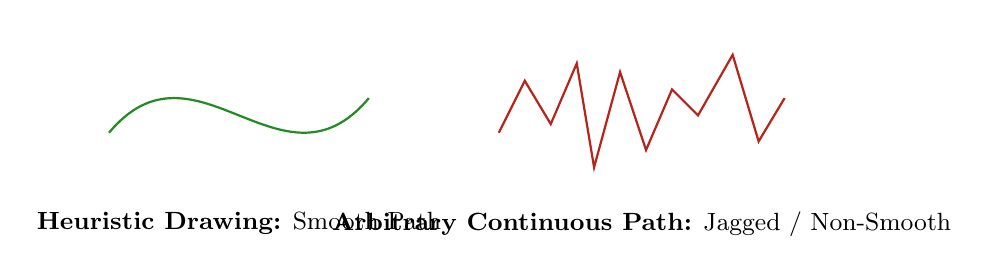
\begin{tikzpicture}[scale=1.1]
    % \begin{hidden}
    % - Canvas: scale 1.1, two curves side by side
    % - Left: Smooth curve; Right: Jagged fractal-like continuous curve
    % - Order: (1) smooth curve; (2) rough zigzag curve; (3) annotations
    % \end{hidden}
    % Smooth curve
    \draw[thick, ForestGreen] (-4, 0) .. controls (-3, 1.2) and (-2, -0.8) .. (-1, 0.4);
    \node[below, font=\small] at (-2.5, -0.8) {\textbf{Heuristic Drawing:} Smooth Path};

    % Rough zigzag curve (stock market analogy)
    \draw[thick, BrickRed] (0.5, 0) -- (0.8, 0.6) -- (1.1, 0.1) -- (1.4, 0.8) -- (1.6, -0.4)
                         -- (1.9, 0.7) -- (2.2, -0.2) -- (2.5, 0.5) -- (2.8, 0.2) -- (3.2, 0.9)
                         -- (3.5, -0.1) -- (3.8, 0.4);
    \node[below, font=\small] at (2.15, -0.8) {\textbf{Arbitrary Continuous Path:} Jagged / Non-Smooth};
\end{tikzpicture}
\end{center}

\begin{steps}[Topological vs. Differential Curves]
A curve $\gamma \colon [0, 1] \to X$ in a general metric space only requires topological continuity, not differentiability (which is not even defined in abstract metric spaces). Thus, continuous curves can exhibit fractal-like, nowhere-differentiable behavior (analogous to Brownian motion or financial stock market trajectories). For pedagogical visualization, we draw smooth arcs, as the topological connectedness properties remain identical.
\end{steps}
\end{content}

\subsection{Definition of Path Connectedness}

\begin{speech}[00:35:42 - 00:37:27]
Another definition, a very nice one, is the notion of path connected \inlinemetanote{writes Def'n (path connectedness)}:

As always, $(X, d)$ is a metric space \inlinemetanote{writes $(X, d)$ m.s.}.

And $E \subset X$ is a set \inlinemetanote{writes $E \subset X$ set}.

It is called path connected \inlinemetanote{writes is called path connected} if, for every pair of points $x, y$ in my set \inlinemetanote{writes if $\forall x, y \in E$}, there exists a path joining $x$ and $y$ \inlinemetanote{writes $\exists \text{ path joining } x \text{ and } y$}.

More precisely, given the two points $x$ and $y$, there exists some $\gamma$ from $[0, 1]$ to $E$ continuous \inlinemetanote{writes $\implies \exists \gamma \colon [0, 1] \to E \text{ continuous}$} such that $\gamma(0) = x$ and $\gamma(1) = y$ \inlinemetanote{writes s.t. $\gamma(0) = x, \ \gamma(1) = y$}.
\end{speech}

\begin{speech}[00:37:27 - 00:38:25]
Again, the same drawing: if my set $E$ is like this, and I take the point $x$ here and $y$ here \inlinemetanote{draws a disconnected set $E$ consisting of two separate components, with $x$ in one component and $y$ in the other}, there is no way I'm going to find a continuous curve --- at least intuitively --- that goes from this point to this point without exiting my set \inlinemetanote{draws a curve between $x$ and $y$ that exits $E$}, right?

Because the curve would need to go here, and then jump to this point. And continuous curves --- this is the point --- cannot jump.

But this is an intuition. Now we will need to see what is the connection or the relation between connectedness and path connectedness, right? There is some relation.
\end{speech}

\begin{content}
\begin{definition}[Path Connected Set]\label[definition]{def:path-connectedness}
Let $(X, d)$ be a metric space. A subset $E \subseteq X$ is called \newterm{path connected} if for every pair of points $x, y \in E$, there exists a path within $E$ connecting them. That is:
\begin{equation}\label{eq:path-connected-def}
\forall x, y \in E, \quad \exists \gamma \colon [0, 1] \to E \text{ continuous such that } \gamma(0) = x \text{ and } \gamma(1) = y.
\end{equation}
\end{definition}

\begin{center}
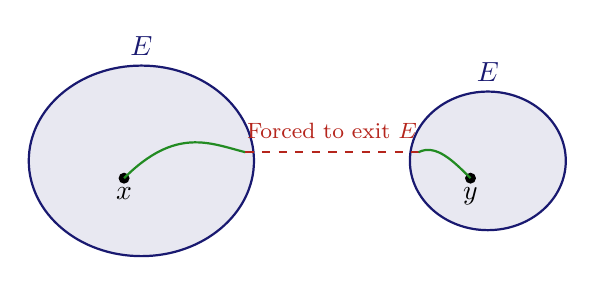
\begin{tikzpicture}[scale=1.1]
    % \begin{hidden}
    % - Canvas: scale 1.1, two disjoint components of E
    % - Order: (1) component E_1; (2) component E_2; (3) points x and y;
    %   (4) continuous curve forced to leave E; (5) labels
    % - Coordinates: E_1 centered at (-2, 0), radius 1.2; E_2 centered at (2, 0), radius 0.9.
    %   x at (-1.8, -0.2); y at (1.8, -0.2).
    % - Path: solid within E_1 and E_2, dashed in the exterior gap.
    % - Labels: x, y, E, and note on jumping.
    % \end{hidden}
    % Component 1 of E
    \draw[thick, MidnightBlue, fill=MidnightBlue!10] (-2, 0) ellipse (1.3 and 1.1);
    \node[MidnightBlue, above] at (-2, 1.1) {$E$};

    % Component 2 of E
    \draw[thick, MidnightBlue, fill=MidnightBlue!10] (2, 0) ellipse (0.9 and 0.8);
    \node[MidnightBlue, above] at (2, 0.8) {$E$};

    % Points x and y
    \fill[black] (-2.2, -0.2) circle (1.8pt) node[below] {$x$};
    \fill[black] (1.8, -0.2) circle (1.8pt) node[below] {$y$};

    % Attempted connecting curve
    \draw[thick, ForestGreen] (-2.2, -0.2) .. controls (-1.6, 0.4) and (-1.2, 0.2) .. (-0.8, 0.1);
    \draw[thick, dashed, BrickRed] (-0.8, 0.1) -- (1.2, 0.1);
    \draw[thick, ForestGreen] (1.2, 0.1) .. controls (1.4, 0.2) and (1.6, 0.0) .. (1.8, -0.2);

    \node[BrickRed, font=\footnotesize, above] at (0.2, 0.15) {Forced to exit $E$};
\end{tikzpicture}
\end{center}

\begin{steps}[Key Distinction: Path in the Subset]
Notice that the definition of path connectedness explicitly requires the codomain of the path to be $E$ itself ($\gamma \colon [0, 1] \to E$), rather than the ambient space $X$. In a disconnected set composed of separate pieces, any continuous path attempting to link points in different components must exit the set, violating $\gamma([0, 1]) \subseteq E$.
\end{steps}
\end{content}

\subsection{Path Connectedness Implies Connectedness}

\begin{speech}[00:38:25 - 00:39:05]
There is one relation that works always, that is the following proposition \inlinemetanote{writes Prop}.

Proposition: Again, in a general metric space \inlinemetanote{writes $(X, d)$ m.s.}, $E$ is path connected \inlinemetanote{writes $E$ is path connected} implies that $E$ is connected \inlinemetanote{writes $\implies E$ connected}.

So, this is the easy implication. And this is always true, right?

\inlinemetanote{writes proof}
\end{speech}

\begin{content}
\begin{proposition}[Path Connectedness Implies Connectedness]\label[proposition]{prop:path-connected-implies-connected}
Let $(X, d)$ be a metric space. If a subset $E \subseteq X$ is path connected, then $E$ is connected:
\begin{equation}\label{eq:path-connected-implies-connected}
E \subseteq X \text{ path connected} \implies E \text{ connected}.
\end{equation}
\end{proposition}
\end{content}

\begin{hidden}
% timestamp: 00:18:48
% topic: Proof that Path Connectedness Implies Connectedness
% board_state: prop:path-connected-implies-connected, eq:path-connected-implies-connected
% next_goal: Prove by contraposition: Assume E disconnected, show not path connected
% open_loops: none
\end{hidden}

\begin{proofWrapper}[Proof of \cref{prop:path-connected-implies-connected}]

\begin{speech}[00:39:05 - 00:40:24]
Proof.

I know that there are many new techniques and ideas, but now they start to repeat themselves many times, no?

How do I prove this implication? Well, it's good to work with disconnected, so I will prove by contraposition. I will say:

Assume that $E$ is disconnected \inlinemetanote{writes proof: Assume that $E$ is disconnected}, right?

Then this implies that there exist $U_1, U_2$ open, disjoint \inlinemetanote{writes $\implies \exists U_1, U_2 \text{ open disjoint}$} such that $E$ is contained in the union \inlinemetanote{writes $E \subset U_1 \cup U_2$}, and both of them have non-empty intersection. This means that there exists a point $x_i$ in $U_i$ intersected with $E$ \inlinemetanote{writes $\exists x_i \in U_i \cap E$}.

This I said three times today, so this part should be okay.
\end{speech}

\begin{content}[Contraposition Setup]
We prove the statement by contraposition:
\[
E \text{ is disconnected} \implies E \text{ is not path connected}.
\]
Assume $E$ is disconnected. By \cref{def:disconnected-and-connected-sets}, there exist open sets $U_1, U_2 \subseteq X$ such that:
\begin{align}
U_1 \cap U_2 &= \emptyset && \text{(disjoint),} \label{eq:prop-u-disjoint} \\
E &\subseteq U_1 \cup U_2 && \text{(covering $E$),} \label{eq:prop-u-cover} \\
U_i \cap E &\neq \emptyset \quad \text{for } i \in \{1, 2\} && \text{(non-empty intersections).} \label{eq:prop-u-nonempty}
\end{align}
In particular, by \eqref{eq:prop-u-nonempty}, we can choose points $x_1 \in U_1 \cap E$ and $x_2 \in U_2 \cap E$.
\end{content}

\begin{speech}[00:40:24 - 00:41:35]
And now we want to contradict that this $E$ is path connected.

Assume by contradiction \inlinemetanote{writes Assume by contr.} that there was a map, that there exists a $\gamma$ \inlinemetanote{writes $\exists \gamma$}, a curve joining $x_1$ and $x_2$ \inlinemetanote{writes joining $x_1$ and $x_2$}, right?

What does it mean? This means that $\gamma$ from $[0, 1]$ to $E$ \inlinemetanote{writes $\gamma \colon [0, 1] \to E$} would be continuous \inlinemetanote{writes continuous}, right? And then $\gamma(0)$ would be $x_1$ and $\gamma(1)$ would be $x_2$ \inlinemetanote{writes $\gamma(0) = x_1, \ \gamma(1) = x_2$}.
\end{speech}

\begin{content}[Hypothesis of a Connecting Path]
Suppose for contradiction that $E$ is path connected.
Then there exists a continuous path joining $x_1$ and $x_2$ within $E$:
\begin{equation}\label{eq:connecting-path-gamma}
\gamma \colon [0, 1] \to E \quad \text{continuous with} \quad \gamma(0) = x_1 \quad \text{and} \quad \gamma(1) = x_2.
\end{equation}
\end{content}

\begin{speech}[00:41:35 - 00:43:15]
But $U_1$ and $U_2$ are open sets, so we can do the preimage of those open sets by $\gamma$, and this would give me... Now I can consider: how do I call them?

I can call them $V_i = \gamma^{-1}(U_i)$ \inlinemetanote{writes $V_i = \gamma^{-1}(U_i)$}, right?

These are subsets of $[0, 1]$ \inlinemetanote{writes $\subset [0, 1]$}, right? And $[0, 1]$ as a metric space.

These would be two subsets of $[0, 1]$ that are relatively open --- this means open as subsets of this \inlinemetanote{writes open} ---, disjoint \inlinemetanote{writes disjoint}, and covering $[0, 1]$ \inlinemetanote{writes and covering $[0, 1]$}.

And each of them has a point, because one has the zero, and one has the one.

So, this would prove \inlinemetanote{writes $\implies$} that $[0, 1]$ is disconnected \inlinemetanote{writes $[0, 1]$ disconnected}.

But we know, because we proved before, that intervals are connected. So, this is a contradiction \inlinemetanote{writes contradiction}.
\end{speech}

\begin{content}[Pullback Disconnection of the Unit Interval]
We define the pullbacks of $U_1$ and $U_2$ under $\gamma$ in the unit interval $[0, 1]$:
\begin{equation}\label{eq:v-pullbacks-interval}
V_1 := \gamma^{-1}(U_1) \quad \text{and} \quad V_2 := \gamma^{-1}(U_2).
\end{equation}
We examine the topological properties of $V_1, V_2 \subseteq [0, 1]$:
\begin{itemize}
    \item \textbf{Openness:} Since $U_1, U_2$ are open in $X$ and $\gamma \colon [0, 1] \to X$ is continuous, $V_1, V_2$ are open in the subspace topology of $[0, 1]$.
    \item \textbf{Disjointness:} Since $U_1 \cap U_2 = \emptyset$:
    \[
    V_1 \cap V_2 = \gamma^{-1}(U_1) \cap \gamma^{-1}(U_2) = \gamma^{-1}(U_1 \cap U_2) = \gamma^{-1}(\emptyset) = \emptyset.
    \]
    \item \textbf{Covering $[0, 1]$:} Since $\gamma([0, 1]) \subseteq E \subseteq U_1 \cup U_2$:
    \[
    [0, 1] = \gamma^{-1}(\gamma([0, 1])) \subseteq \gamma^{-1}(U_1 \cup U_2) = \gamma^{-1}(U_1) \cup \gamma^{-1}(U_2) = V_1 \cup V_2.
    \]
    \item \textbf{Non-Emptiness:} Since $\gamma(0) = x_1 \in U_1$, we have $0 \in V_1 \neq \emptyset$. Similarly, since $\gamma(1) = x_2 \in U_2$, we have $1 \in V_2 \neq \emptyset$.
\end{itemize}
Thus, the pair $(V_1, V_2)$ disconnects the unit interval $[0, 1]$:
\[
[0, 1] \text{ is disconnected.}
\]
However, by \cref{prop:connected-subsets-r}, any interval in $\mathbb{R}$ is connected. This is a \textbf{contradiction}.
Hence, no such continuous path $\gamma$ can exist in $E$.
Therefore, $E$ cannot be path connected.
By contraposition, if $E$ is path connected, then $E$ is connected.
\end{content}

\begin{speech}[00:43:15 - 00:43:48]
You see, the contradiction comes from the assumption that there is a continuous path joining the points $x_1$ and $x_2$ that are here in different, disjoint open sets.

So, this is almost a variation of the proof I gave before, right? That the image of a connected set is connected. \inlinemetanote{draws $\square$ on the board}
\end{speech}

\end{proofWrapper}

\section{Distinction Between Connectedness and Path Connectedness}

\subsection{A Connected Set That Is Not Path Connected: The Topologist's Sine Curve}

\begin{speech}[00:43:48 - 00:45:11]
Okay, so let's continue.

Now we know that in a general metric space, a path connected subset must be connected, right?

But intuitively it looks like the two notions are defining the same type of property. So, what is the difference between the two? When are they equivalent? When are they not?

First I will give you the book example of a set that is connected, but is not path connected, okay? This is a book example. You don't encounter such sets in life very often, but they exist, right?

So, we will take $\mathbb{R}^2$ with the Euclidean distance \inlinemetanote{writes $(\mathbb{R}^2, d_{\text{Eucl}})$}.

Why do I need to go to $\mathbb{R}^2$? Because in $\mathbb{R}$, we just proved that connected sets are the same as intervals, and that is the same as path connected. In $\mathbb{R}$, everything is very trivial. But when you go to $\mathbb{R}^2$, you have two directions to play with and things are more interesting.
\end{speech}

\begin{speech}[00:45:11 - 00:46:41]
The book example is this set:

This would be $y$ and $x$ \inlinemetanote{draws $y$-axis and $x$-axis}. And we will take the set $E$ to be this interval \inlinemetanote{writes $E =$}, this interval over here, right? \inlinemetanote{draws a red vertical segment on the $y$-axis} The interval $\{0\} \times [0, 1]$ \inlinemetanote{writes $\{0\} \times [0, 1]$}, this vertical interval, and then the union of the points $(t, \sin(1/t))$ where $t$ is a positive number \inlinemetanote{writes $\cup \{ (t, \sin(1/t)) \mid t > 0 \}$}.

This is like a curve. You see, $t$ is positive, so I'm parametrizing this curve. When $t$ is very large, $\sin(1/t)$ is very slow. But when $t$ goes to zero, $\sin(1/t)$ will start to oscillate like crazy.

And then it will go like this: here will be super slow, and as you approach zero, it will start to oscillate more and more and more and more and more and more and more \inlinemetanote{draws oscillating sine wave approaching the $y$-axis}.
\end{speech}

\begin{content}[The Topologist's Sine Curve: Preliminary Definition]
In the Euclidean plane $(\mathbb{R}^2, d_{\text{Eucl}})$, consider the preliminary set:
\[
E_{\text{prelim}} := \left( \{0\} \times [0, 1] \right) \cup \left\{ \left( t, \sin\left(\frac{1}{t}\right)\right) \;\middle|\; t > 0 \right\}.
\]
\end{content}

\begin{speech}[00:46:41 - 00:47:25]
Well, do I want to do this? Yes, but then maybe I want to take $[-1, 1]$. Then... \inlinemetanote{corrects $[0, 1]$ to $[-1, 1]$ on the board}

So this would be... yeah. This should hopefully be $1$, and this $-1$ \inlinemetanote{labels $1$ and $-1$ on the $y$-axis and extends the red vertical segment down to $-1$}, and the sine oscillates between these two values, right? And you include all this line.
\end{speech}

\begin{hidden}
% timestamp: 00:06:50
% topic: Counterexample: Topologist's Sine Curve (Connected but not path connected)
% board_state: ex:topologists-sine-curve
% next_goal: Detail heuristics for why it is connected and why path connectedness fails
% open_loops: none
\end{hidden}

\begin{content}
\begin{example}[Topologist's Sine Curve]\label[example]{ex:topologists-sine-curve}
In the Euclidean space $(\mathbb{R}^2, d_{\text{Eucl}})$, the \newterm{topologist's sine curve} is the subset $E \subset \mathbb{R}^2$ defined by:
\begin{equation}\label{eq:topologists-sine-curve-def}
E := \left( \{0\} \times [-1, 1] \right) \cup \left\{ \left( t, \sin\left(\frac{1}{t}\right) \right) \;\middle|\; t > 0 \right\}.
\end{equation}
The set $E$ consists of two parts:
\begin{itemize}
    \item The limiting vertical segment $L := \{0\} \times [-1, 1]$ on the $y$-axis,
    \item The oscillating graph $S := \{ (t, \sin(1/t)) \mid t > 0 \}$.
\end{itemize}
\end{example}

\begin{center}
\begin{tikzpicture}[scale=1.4, >=Stealth]
% \begin{hidden}
% - Canvas: scale 1.4, x in [-0.6, 4.4], y in [-1.6, 1.6]
% - Order: (1) Axes x and y, gray!70; (2) Boundary bounding lines y = 1 and y = -1, dashed gray!40;
%   (3) Dense accumulation lines near x = 0 (simulating infinite oscillations between y = -1 and y = 1);
%   (4) Smooth curve y = sin(1/x) for x in [0.08, 3.8] in ForestGreen;
%   (5) Asymptotic vertical segment on the y-axis from y = -1 to 1 in ultra thick BrickRed;
%   (6) Labels and annotations.
% - Coordinates: x = 0.08 to 3.8:
%   At x = 3.5, 1/x = 0.286 rad ~ 16.4 deg, sin(1/x) ~ 0.28
%   At x = 2/pi ~ 0.637, sin(1/x) = 1
%   At x = 2/(3pi) ~ 0.212, sin(1/x) = -1
%   At x = 2/(5pi) ~ 0.127, sin(1/x) = 1
%   Dense zigzag lines below x = 0.08: x = 0.065, 0.052, 0.042, 0.033, 0.025, 0.018, 0.012
% - Labels: y at (0, 1.6), x at (4.2, 0); ticks 1 at (0, 1) and -1 at (0, -1);
%   Segment label "{0} x [-1, 1]" left of the y-axis in BrickRed;
%   Graph label "(t, sin(1/t))" above the curve peak near x = 0.64 in ForestGreen.
% - Collisions: None; the segment label is at x = -0.15 anchored east, graph label at y = 1.25.
% \end{hidden}
    % Axes
    \draw[->, thick, gray!70] (-0.5, 0) -- (4.2, 0) node[right, text=black] {$x$};
    \draw[->, thick, gray!70] (0, -1.5) -- (0, 1.5) node[above, text=black] {$y$};

    % Dashed envelope lines at y = 1 and y = -1
    \draw[dashed, gray!40] (0, 1) -- (3.8, 1);
    \draw[dashed, gray!40] (0, -1) -- (3.8, -1);

    % Ticks on y-axis
    \draw[thick] (-0.08, 1) -- (0.08, 1) node[left=4pt, font=\small] {$1$};
    \draw[thick] (-0.08, -1) -- (0.08, -1) node[left=4pt, font=\small] {$-1$};

    % Infinite oscillation accumulation near x = 0 (drawn as dense oscillating wave)
    \draw[thick, ForestGreen] 
        (0.012, 0.0) -- (0.015, 0.9) -- (0.020, -0.9) -- (0.026, 0.95) -- (0.034, -0.98) 
        -- (0.045, 0.99) -- (0.060, -0.99) -- (0.080, 0.98);

    % Smooth plot of sin(1/t) for t in [0.08, 3.8]
    \draw[thick, ForestGreen, domain=0.08:3.8, samples=180] 
        plot (\x, {sin((1/\x)*180/pi)});

    % Vertical limiting segment {0} x [-1, 1] on the y-axis
    \draw[ultra thick, BrickRed] (0, -1) -- (0, 1);
    \node[BrickRed, anchor=east, font=\footnotesize, align=right] at (-0.15, 0.5) {$\{0\} \times [-1, 1]$\\(Limiting Segment)};

    % Curve label
    \node[ForestGreen, anchor=south, font=\footnotesize] at (1.4, 0.8) {$y = \sin\left(\frac{1}{t}\right)$};
\end{tikzpicture}
\end{center}
\end{content}

\begin{speech}[00:47:25 - 00:49:28]
I know that the drawing is very bad, but you can find this everywhere, okay?

So, this is the idea: you take a very oscillating curve, and you put the asymptotic vertical line, no?

Now, this is connected because... I'll tell you the heuristic, and then you need to prove it, hm? Exercise: prove that this is connected.

The idea is that this is a union of two pieces: the curve that is very oscillating --- and this curve is connected, right? Because it's path connected, it's a curve --- and then the last piece, that is the segment.

Now, you cannot separate this vertical segment from the rest of the curve using open sets, because if you try to put any open set that contains this vertical segment, it will meet some chunk of the curve, because it's very dense: this curve is accumulating to this vertical line.

So, you can never disconnect this piece, the oscillating piece, and the vertical segment using open sets.

Yet, if you try to prove that this set is path connected, you will need a continuous curve that connects this point over here in the vertical segment and this point here.

And you will see that this is impossible: you cannot find a continuous curve from the closed interval $[0, 1]$ to here that joins these two points.
\end{speech}

\begin{speech}[00:49:28 - 00:49:58]
And the reason is that if you consider such a curve, because a curve is continuous, right? You would have as endpoints of the curve every point on the vertical line.

See, by continuity, you have sequences approaching along the curve: you would have sequences here approaching this point, and sequences here approaching this point --- all of the points could be approached.

So then the left endpoint of the curve, or the last endpoint of the curve, should be any point in this segment, which is a contradiction.

To do this carefully is a good exercise: to prove that this set is not path connected. Not an easy exercise, but you can do it now.

Okay, so this is the book example of a set... This set is connected and not path connected \inlinemetanote{writes This set is connected and not path connected and boxes the example on the board}.
\end{speech}

\begin{content}[Properties of the Topologist's Sine Curve]
\begin{proposition}[Connectedness vs. Path Connectedness of $E$]\label[proposition]{prop:topologist-sine-curve-properties}
The topologist's sine curve $E \subset \mathbb{R}^2$ satisfies:
\begin{equation}\label{eq:topologist-sine-classification}
E \text{ is connected}, \quad \text{but} \quad E \text{ is not path connected}.
\end{equation}
\end{proposition}

\begin{steps}[Heuristic Justification]
\begin{itemize}
    \item \textbf{Why $E$ is connected:}
    The oscillating piece $S = \{ (t, \sin(1/t)) \mid t > 0 \}$ is the continuous image of the connected interval $(0, \infty)$ under the continuous map $t \mapsto (t, \sin(1/t))$. Hence, $S$ is connected.
    The vertical segment $L = \{0\} \times [-1, 1]$ consists entirely of accumulation points of $S$ (since for any $y_0 \in [-1, 1]$, the sequence $t_k = \frac{1}{\arcsin(y_0) + 2\pi k} \to 0^+$ gives $(t_k, \sin(1/t_k)) = (t_k, y_0) \to (0, y_0)$).
    Thus, $E \subseteq \overline{S}$. Since any set sandwiched between a connected set and its topological closure is connected ($S \subseteq E \subseteq \overline{S}$), $E$ is connected.
    Any open set containing $L$ necessarily intersects infinitely many oscillations of $S$, making topological separation by disjoint open sets impossible.

    \item \textbf{Why $E$ is not path connected:}
    Suppose there were a continuous path $\gamma \colon [0, 1] \to E$ connecting a point on $L$, say $(0, 0)$, to a point on $S$, say $(1, \sin(1))$.
    Let $t_0 = \sup \{ t \in [0, 1] \mid \gamma(t) \in L \}$. By continuity of $\gamma$, $\gamma(t_0) \in L$. For $t > t_0$, $\gamma(t) \in S$.
    Writing $\gamma(t) = (\gamma_x(t), \gamma_y(t))$, we have $\gamma_x(t) \to 0^+$ as $t \to t_0^+$.
    However, the $y$-component must satisfy $\gamma_y(t) = \sin(1/\gamma_x(t))$, which oscillates wildly between $-1$ and $1$ as $\gamma_x(t) \to 0^+$.
    Hence, $\lim_{t \to t_0^+} \gamma_y(t)$ cannot exist, contradicting the continuity of $\gamma$ at $t_0$.
\end{itemize}
\end{steps}
\end{content}

\section{Equivalence of Connectedness and Path Connectedness for Open Sets in \texorpdfstring{$\mathbb{R}^n$}{R\textasciicircum n}}

\subsection{Theorem Formulation and Equivalence Setup}

\begin{speech}[00:49:58 - 00:51:53]
This being said, you know that in analysis there are always these pathological examples that you need to know, but you also need not to be very worried about them, because life in general is much better than what the counterexamples show, right?

So, this being said, there is a theorem that is, for practical purposes, what we will apply all the time: that when you have in $\mathbb{R}^n$ Euclidean, in the Euclidean space \inlinemetanote{writes Thm $(\mathbb{R}^n, d_{\text{Eucl}})$}, an open subset $U \subset \mathbb{R}^n$ \inlinemetanote{writes $U \subset \mathbb{R}^n$ open} --- for any open set --- $U$ connected is equivalent to $U$ path connected \inlinemetanote{writes $U \text{ connected} \iff U \text{ path connected}$}.

For open sets of Euclidean space, of $\mathbb{R}^n$, right? And this is what we are going to prove now.

Now, this implication was already proven, because it's general: $U$ path connected implies connected we already proved in a much more general setup \inlinemetanote{writes $\Leftarrow \checkmark$}. This implication always works.

And what remains to be shown is that implication \inlinemetanote{writes $\Rightarrow$}: that in $\mathbb{R}^n$, $U$ connected implies $U$ path connected \inlinemetanote{draws a box around $\Rightarrow$}.
\end{speech}

\begin{content}
\begin{theorem}[Connectedness Equals Path Connectedness for Open Sets in $\mathbb{R}^n$]\label[theorem]{thm:connected-open-rn}
Let $U \subseteq \mathbb{R}^n$ be an open subset of the Euclidean space $(\mathbb{R}^n, d_{\text{Eucl}})$.
Then $U$ is connected if and only if $U$ is path connected:
\begin{equation}\label{eq:connected-iff-path-connected-rn}
U \text{ is connected} \iff U \text{ is path connected}.
\end{equation}
\end{theorem}
\end{content}

\begin{proofWrapper}[Proof of \cref{thm:connected-open-rn}]

\subsubsection{Reduction to a Fixed Basepoint}

\begin{speech}[00:51:53 - 00:54:10]
Okay, so goal... \inlinemetanote{writes Goal:}

How will we prove that? We will have our connected set $U$... \inlinemetanote{draws an open connected domain $U$ on the chalkboard}

This $U$, I draw it connected, but just to make the drawing, no? And then I will pick a point $x_0$ in $U$ \inlinemetanote{marks $x_0$ in $U$}.

Pick $x_0$ in $U$ and prove we can join it with any other point $x$ in $U$ by a path \inlinemetanote{writes Pick $x_0 \in U$ and prove we can join it with any other point $x \in U$ by a path, and boxes it in yellow chalk}.

My goal is: I will fix this point, and now I will take any point $x$ here \inlinemetanote{marks point $x$ in $U$}, and I will show that I can always join $x_0$ and $x$ by some path \inlinemetanote{draws a path from $x_0$ to $x$}.

And since this is arbitrary, now you can tell me: okay, is this enough? Why, if you have this, you can join $x$ and $y$, right? Imagine that now you want to join $x$ and $y$ \inlinemetanote{marks point $y$ in $U$}.

So, if I have a path going from $x_0$ to $x$, and another path going from $x_0$ to $y$ \inlinemetanote{draws dashed path from $x_0$ to $y$}, there is always a way to construct a path from $x$ to $y$.

How do you do it? You take the path from $x_0$ to $x$, you reverse it, and then when you finish that, you compound it with the other path.
\end{speech}

\begin{hidden}
% timestamp: 00:12:00
% topic: Equivalence of Connectedness and Path Connectedness for Open Sets in R^n
% board_state: thm:connected-open-rn, goal-basepoint
% next_goal: Define path operations (reversal and composition) to justify the basepoint reduction
% open_loops: none
\end{hidden}

\begin{content}[Reduction to Connecting to a Fixed Basepoint]
The implication $U \text{ path connected} \implies U \text{ connected}$ holds in every metric space by \cref{prop:path-connected-implies-connected}.
It remains to prove the forward direction:
\[
U \subseteq \mathbb{R}^n \text{ open and connected} \implies U \text{ is path connected}.
\]

\begin{highlight}{BurntOrange}[Goal Formulation via Fixed Basepoint]
Fix an arbitrary basepoint $x_0 \in U$. We claim that it suffices to prove:
\begin{equation}\label{eq:yellow-goal}
\forall x \in U, \quad \exists \text{ path in } U \text{ joining } x_0 \text{ to } x.
\end{equation}
\end{highlight}

\begin{center}
\begin{tikzpicture}[scale=1.2, >=Stealth]
    % \begin{hidden}
    % - Canvas: scale 1.2, x in [-3, 4], y in [-2, 2.2]
    % - Order: (1) Domain U, thick MidnightBlue line with light fill MidnightBlue!5;
    %   (2) Basepoint x_0 in the interior;
    %   (3) Points x and y in U;
    %   (4) Path gamma_x from x_0 to x in ForestGreen;
    %   (5) Path gamma_y from x_0 to y in BurntOrange (dashed);
    %   (6) Resulting path from x to y via x_0 indicated.
    % - Coordinates: x_0 = (-1.2, 0.2), x = (1.5, 0.9), y = (1.2, -0.9)
    % - Labels: U above right at (2.8, 1.4); x_0 below-left; x above; y below;
    %   gamma_x above its curve; gamma_y below its curve.
    % \end{hidden}
    % Ambient open domain U
    \draw[thick, MidnightBlue, fill=MidnightBlue!5] 
        (-2.2, 0) .. controls (-2.0, 1.5) and (-0.5, 1.8) .. (0.8, 1.2)
                 .. controls (1.8, 0.8) and (2.2, 1.8) .. (3.0, 1.0)
                 .. controls (3.6, 0.2) and (3.0, -1.2) .. (2.0, -1.5)
                 .. controls (0.8, -1.8) and (-0.5, -0.8) .. (-1.5, -1.4)
                 .. controls (-2.4, -1.2) and (-2.4, -0.5) .. (-2.2, 0) -- cycle;
    \node[MidnightBlue, font=\large\bfseries] at (2.8, 1.4) {$U$};

    % Points
    \coordinate (X0) at (-1.2, 0.2);
    \coordinate (X) at (1.5, 0.9);
    \coordinate (Y) at (1.2, -0.9);

    \fill[black] (X0) circle (2pt) node[below left=2pt] {$x_0$};
    \fill[BrickRed] (X) circle (2pt) node[above=2pt, BrickRed] {$x$};
    \fill[BrickRed] (Y) circle (2pt) node[below=2pt, BrickRed] {$y$};

    % Path from x_0 to x (gamma_1)
    \draw[ultra thick, ForestGreen] 
        (X0) .. controls (-0.5, 0.6) and (0.5, 0.4) .. (X);
    \node[ForestGreen, font=\footnotesize, above] at (0.2, 0.6) {$\gamma_x$};

    % Path from x_0 to y (gamma_2)
    \draw[ultra thick, dashed, BurntOrange] 
        (X0) .. controls (-0.6, -0.4) and (0.4, -0.2) .. (Y);
    \node[BurntOrange, font=\footnotesize, below] at (0.2, -0.4) {$\gamma_y$};
\end{tikzpicture}
\end{center}

\begin{steps}[Why Connecting to a Basepoint Suffices]
If every point in $U$ can be joined to the fixed point $x_0$, then for any two points $x, y \in U$:
\begin{enumerate}[label=\textbf{(\arabic*)}]
    \item There exists a path $\gamma_x$ from $x_0$ to $x$.
    \item There exists a path $\gamma_y$ from $x_0$ to $y$.
\end{enumerate}
By reversing $\gamma_x$ (running backwards from $x$ to $x_0$) and concatenating it with $\gamma_y$ (running from $x_0$ to $y$), we obtain a continuous path running from $x$ to $y$ entirely within $U$.
\end{steps}
\end{content}

\subsubsection{Operations on Paths: Reversal and Composition}

\begin{speech}[00:54:10 - 00:55:55]
Let me write this analytically. This is the composition of paths.

Composing paths \inlinemetanote{writes Composing paths} is something that I will use in this proof many times.

It says: if $\gamma_1$ from $[0, 1]$ to $X$ \inlinemetanote{writes $\gamma_1 \colon [0, 1] \to X$} satisfies that $\gamma_1(0) = x$ \inlinemetanote{writes $\gamma_1(0) = x$} and $\gamma_1(1) = y$ \inlinemetanote{writes $\gamma_1(1) = y$}... Let me call this first path $\gamma_1$.

And the second path, $\gamma_2$, is a path from $[0, 1]$ to $X$ \inlinemetanote{writes $\gamma_2 \colon [0, 1] \to X$} joining $y$ and $z$ \inlinemetanote{writes $\gamma_2(0) = y, \ \gamma_2(1) = z$}, right?

Let me do the drawing again. This is my abstract space $X$ \inlinemetanote{draws boundary of $X$}, and I have a path going from $x$ to $y$ \inlinemetanote{draws path from $x$ to $y$} --- this is $\gamma_1$ --- and another path going from $y$ to $z$ \inlinemetanote{draws path from $y$ to $z$}.

The arrow is the direction of motion \inlinemetanote{draws directional arrow on $\gamma_1$}, and this is $\gamma_2$ \inlinemetanote{draws directional arrow on $\gamma_2$}, right?
\end{speech}

\begin{speech}[00:55:55 - 00:57:45]
Then I can always do an operation. I can first reverse any of the paths. I can define $\gamma_1$ reversed \inlinemetanote{writes $\gamma_1^* \text{ (reversed)}$} --- let's say $\gamma_1^*$, to call it something. This is the reversed path, that is defined as $\gamma_1^*(t) = \gamma_1(1 - t)$ \inlinemetanote{writes $\gamma_1^*(t) = \gamma(1 - t)$}.

You see, this is composing $\gamma_1$ with a map that is also continuous, right? The composition of continuous maps will be continuous.

By the way, exercise: show this \inlinemetanote{writes [Show comp. of continuous maps is cont.]}. Show that the composition of continuous maps is continuous.

Now you will see that you know many tools to show things very quickly, because if I want to show that the composition of continuous maps is continuous, I can check: okay, what is my definition of continuous? Preimage of an open set is an open set.

So, if I take two preimages: preimage of an open set is an open set, preimage of an open set is an open set, and I'm done, right?

So now it's very easy to prove many things when you have a lot of equivalent definitions of continuity, for instance.

If you believe me that the composition of continuous maps is continuous, this is a new continuous map from $[0, 1]$ to $X$, and you see that now it is going from $y$ to $x$, because you are going backwards in time. Yeah.
\end{speech}

\begin{student}[Student Question]
The length?
\end{student}

\begin{speech}[00:58:09 - 00:58:35]
The length? Yeah, we will see the length, but not yet. The length is a property mainly of differentiable paths, or piecewise differentiable paths.

For a continuous path, the length can be very large; it can be infinite. But we will define the length later on.
\end{speech}

\begin{speech}[00:58:35 - 01:00:18]
So, this is just reversing the path. And what you can always do is compose the two paths, right?

You can do the composition, let's say $\gamma_3$ \inlinemetanote{writes $\gamma_3(t) =$}. And how do you do the composition?

Okay, you say: for $t$ between $0$ and $1/2$ \inlinemetanote{writes $t \in [0, 1/2]$}, I will take $\gamma_1(2t)$ \inlinemetanote{writes $\gamma_1(2t)$}, right?

And for $t$ between $1/2$ and $1$ \inlinemetanote{writes $t \in [1/2, 1]$}, I will define $\gamma_3$ as $\gamma_2(2t - 1)$ \inlinemetanote{writes $\gamma_2(2t - 1)$}.

And if you think of what it's doing, this is doing this first path $\gamma_1$ at twice the speed. Now you will tell me: you don't know what the speed is in this context. But I'm just saying intuitively what it's doing --- this is informal language.

So, you are doing this path at twice the speed, and this path at twice the speed, and then in one second you are joining $x$ to $z$. So this is the composition of paths, right?

Given any path, you can do the inverse and the composition of paths.

And that's why, whenever you can join $x_0$ to $x$ and $x_0$ to $y$, you can also join $x$ to $y$. You just do the composition of the inverse of this and this, okay? Is this clear? It is intuitive also.
\end{speech}

\begin{hidden}
% timestamp: 00:18:00
% topic: Path concatenation and speed doubling
% board_state: def:path-reversal, def:path-composition
% next_goal: Prove that the path-reachable component G is open and closed in U
% open_loops: student question on path continuity at t = 1/2
\end{hidden}

\begin{content}
\begin{definition}[Reversed Path]\label[definition]{def:reversed-path}
Let $\gamma \colon [0, 1] \to X$ be a continuous path from $x$ to $y$. The \newterm{reversed path} $\gamma^* \colon [0, 1] \to X$ is defined by:
\begin{equation}\label{eq:reversed-path-def}
\gamma^*(t) := \gamma(1 - t).
\end{equation}
The path $\gamma^*$ is continuous and runs from $y = \gamma^*(0)$ to $x = \gamma^*(1)$.
\end{definition}

\begin{definition}[Composition / Concatenation of Paths]\label[definition]{def:path-composition}
Let $\gamma_1 \colon [0, 1] \to X$ be a path with $\gamma_1(0) = x, \ \gamma_1(1) = y$, and let $\gamma_2 \colon [0, 1] \to X$ be a path with $\gamma_2(0) = y, \ \gamma_2(1) = z$.
The \newterm{concatenated path} $\gamma_3 = \gamma_1 * \gamma_2 \colon [0, 1] \to X$ is defined by:
\begin{equation}\label{eq:path-composition-def}
\gamma_3(t) := \begin{cases}
\gamma_1(2t) & \text{if } t \in [0, 1/2], \\[4pt]
\gamma_2(2t - 1) & \text{if } t \in [1/2, 1].
\end{cases}
\end{equation}
\end{definition}

\begin{center}
\begin{tikzpicture}[scale=1.2, >=Stealth]
    % \begin{hidden}
    % - Canvas: scale 1.2, x in [-2.5, 4.5], y in [-1.5, 2]
    % - Order: (1) Ambient space X in MidnightBlue!40;
    %   (2) Points x, y, z;
    %   (3) Path gamma_1 from x to y with arrow;
    %   (4) Path gamma_2 from y to z with arrow;
    %   (5) Labels.
    % - Coordinates: x = (-1.5, -0.2), y = (0.5, 1.2), z = (2.8, -0.3)
    % \end{hidden}
    \draw[thick, gray!60] (-2.2, -1.2) rectangle (3.8, 1.8);
    \node[gray!80, font=\large\bfseries] at (3.5, 1.5) {$X$};

    \coordinate (Px) at (-1.5, -0.2);
    \coordinate (Py) at (0.5, 1.1);
    \coordinate (Pz) at (2.6, -0.3);

    \fill[black] (Px) circle (2pt) node[left=2pt] {$x$};
    \fill[black] (Py) circle (2pt) node[above=2pt] {$y$};
    \fill[black] (Pz) circle (2pt) node[right=2pt] {$z$};

    \draw[->, ultra thick, ForestGreen] 
        (Px) .. controls (-1.0, 0.8) and (-0.2, 1.2) .. (Py);
    \node[ForestGreen, above left] at (-0.3, 0.8) {$\gamma_1$};

    \draw[->, ultra thick, BurntOrange] 
        (Py) .. controls (1.2, 1.0) and (2.0, 0.5) .. (Pz);
    \node[BurntOrange, above right] at (1.6, 0.8) {$\gamma_2$};
\end{tikzpicture}
\end{center}

\begin{steps}[Kinematic Intuition of Concatenation]
The piecewise formula traverses the first path $\gamma_1$ on the time interval $[0, 1/2]$ at double speed ($2t$), arriving at the junction point $\gamma_1(1) = y$ at $t = 1/2$. On $[1/2, 1]$, it traverses $\gamma_2$ at double speed ($2t - 1$), starting at $\gamma_2(0) = y$ at $t = 1/2$ and terminating at $\gamma_2(1) = z$ at $t = 1$.
\end{steps}
\end{content}

\subsubsection{Proof of Path Reachability via Connectedness of the Base Component}

\begin{speech}[01:00:18 - 01:01:53]
Okay, so now we need to prove our goal over here.

And now we will see a strategy of proof that will appear at least three times in this course. At least three times! It's very typical. And I would say that the first time you see it, it looks super smart, this strategy of proof.

Later, when you see it three times, it starts to appear more natural. But it's a nice strategy of proof.

It's how you use in practice the assumption of connectedness.

Remember that we have a set that is connected, and we want to use this assumption of connectedness to prove that it is path connected. How will you use the assumption of connectedness in practice to derive a conclusion?

So, we will do that: we will define... Proof of the yellow claim, proof of that \inlinemetanote{writes proof [box]}.
\end{speech}

\begin{student}[Student Question]
Uh, so, if you take the $\gamma_1$ and $\gamma_2$ and you just put one-half in, it seems like you don't get the same result, so I'm confused about that.
\end{student}

\begin{speech}[01:02:05 - 01:02:44]
So, if you put... You mean here?

For this path to be continuous, what do you need? At the point $1/2$, you need to get the same. This is what you're asking.

But you see, if you put $t = 1/2$, you get $\gamma_1(1)$, and $\gamma_1(1)$ was $y$.

And if you put $\gamma_2(1/2)$, you get $\gamma_2(0)$, that is also $y$.
\end{speech}

\begin{student}[Student Response]
Okay, thank you.
\end{student}

\begin{speech}[01:02:45 - 01:03:02]
The two paths are correctly compounded. But it's a fair question, and we checked that it was correct, okay?
\end{speech}

\begin{speech}[01:03:02 - 01:04:40]
Okay, so to prove this, the trick is to define the set...

Define the set $G \subset U$ \inlinemetanote{writes Define set $G \subset U$}.

$G$ is, by definition, the set of points $x \in U$ such that there exists a path $\gamma$ from $[0, 1]$ to $U$ with $\gamma(0) = x_0$ and $\gamma(1) = x$ \inlinemetanote{writes $G := \{ x \in U \mid \exists \text{ path } \gamma \colon [0, 1] \to U \text{ with } \gamma(0) = x_0 \text{ and } \gamma(1) = x \}$}.

The point $x_0$ is fixed throughout the proof; the point $x_0$ will be fixed all the time, it's the same. I picked any point in $U$.

And now I consider a set $G$ that is the set of points that can be joined by a continuous path with the given point $x_0$, right?

And my goal is to prove that $G$ is everything, is the whole $U$ \inlinemetanote{writes goal $G = U$}.

If I prove that $G$ is the whole $U$, I'm happy, because then I prove that any point can be joined to $x_0$, which is what I claimed, right?

And now this is the cool trick: how we use connectedness.
\end{speech}

\begin{content}[Path-Component Set $G$ and Proof Goal]
Fix an arbitrary basepoint $x_0 \in U$. We define the set of points in $U$ that can be connected to $x_0$ via a continuous path in $U$:
\begin{equation}\label{eq:def-component-g}
G := \left\{ x \in U \;\middle|\; \exists \text{ path } \gamma \colon [0, 1] \to U \text{ such that } \gamma(0) = x_0 \text{ and } \gamma(1) = x \right\}.
\end{equation}

\textbf{Goal:} Prove that $G = U$.
\end{content}

\begin{speech}[01:04:40 - 01:06:17]
So, what we will prove is that:

First, $G$ is open \inlinemetanote{writes 1) $G$ open}. We will prove that $G$ is open.

And we will prove that the complement of $G$, $U \setminus G$, is also open \inlinemetanote{writes 2) $U \setminus G$ open}.

And you see that $G$ always contains the point $x_0$ \inlinemetanote{writes $\ni x_0$ next to 1)}. The point $x_0$ always can be joined by a path that is constant. A constant path is always a nice path. So the point $x_0$ belongs to $G$.

And the only possibility, since $U$ is connected \inlinemetanote{draws a bracket and writes $U$ connected}... Using that $U$ is connected, these two things will imply that $U \setminus G$ is empty \inlinemetanote{writes $\implies U \setminus G = \emptyset$}, right?

A connected set cannot be split as the union of two disjoint non-empty open sets. One of the two needs to be empty; they cannot both be non-empty. This is the very definition of connected, okay?

This is how the strategy goes. So, I need to prove \textbf{1)} and \textbf{2)}: that $G$ is open, and that $U \setminus G$ is open.
\end{speech}

\begin{content}[Proof Strategy: Clopen Components in a Connected Set]
To show that $G = U$, we demonstrate that $G$ is both open and closed in the relative topology of $U$ (a \newterm{clopen} subset of $U$):
\begin{enumerate}[label=\textbf{\arabic*)}]
    \item $G$ is open in $\mathbb{R}^n$, with $x_0 \in G$ (via the constant path $\gamma(t) \equiv x_0$).
    \item $U \setminus G$ is open in $\mathbb{R}^n$.
\end{enumerate}

\begin{steps}[Reduction via Connectedness]
Since $x_0 \in G$, we have $G \neq \emptyset$. The pair $(G, U \setminus G)$ partitions $U$ into disjoint open sets:
\[
U = G \cup (U \setminus G), \quad G \cap (U \setminus G) = \emptyset.
\]
If $U \setminus G$ were non-empty, $(G, U \setminus G)$ would form a disconnection of $U$, contradicting the hypothesis that $U$ is connected (\cref{def:disconnected-and-connected-sets}). Therefore, we must have:
\[
U \setminus G = \emptyset \implies G = U.
\]
\end{steps}
\end{content}

\begin{hidden}
% timestamp: 00:05:25
% topic: Equivalence of connectedness and path-connectedness for open sets in R^n
% board_state: thm:connected-open-rn, eq:def-component-g
% next_goal: Prove that G and U \setminus G are open using local convexity of balls
% open_loops: none
\end{hidden}

\begin{speech}[01:06:17 - 01:08:17]
And the key observation for both \textbf{1)} and \textbf{2)} \inlinemetanote{writes Key observation for 1), 2)} is that if I take any point... This is my set $U$ \inlinemetanote{draws boundary of $U$}, this is $x_0$, this is $x$, right?

For all $x$ in $U$ \inlinemetanote{writes $\forall x \in U$}, we know that there exists a ball of radius $r$ centered at $x$ that is contained in $U$ \inlinemetanote{writes $\exists B_r(x) \subset U$ for $r > 0$ (because $U$ open)}, right?

This would be the ball of radius $r$ centered at $x$ \inlinemetanote{draws dashed circle $B_r(x)$ around $x$}.

And now, a point $y$ in this ball \inlinemetanote{marks $y \in B_r(x)$}: $y$ in the ball of radius $r$ centered at $x$ belongs to $G$ \inlinemetanote{writes $[ y \in B_r(x) \ (\in G \iff x \in G) ]$} if and only if $x$ belongs to $G$.

This is the key observation.

Give me any point $x$. Give me a ball around it, and there is a $y$. $y$ belongs to $G$ --- that is, $y$ can be connected to $x_0$ --- if and only if $x$ can be connected to $x_0$.

Why so? Because the points in a ball can always be joined by a segment, which is a path.

Why? \inlinemetanote{writes Why}
\end{speech}

\begin{content}[Key Observation: Ball Invariance of Path Reachability]
\textbf{Key Observation for 1) and 2):}
Since $U \subseteq \mathbb{R}^n$ is open, for every $x \in U$, there exists $r > 0$ such that the Euclidean open ball $B_r(x)$ is entirely contained in $U$:
\begin{equation}\label{eq:ball-contained-u}
\forall x \in U, \quad \exists r > 0 \quad \text{such that} \quad B_r(x) \subseteq U.
\end{equation}
Then, for every point $y \in B_r(x)$, we have the equivalence:
\begin{equation}\label{eq:key-observation-equiv}
y \in B_r(x) \implies \bigl( y \in G \iff x \in G \bigr).
\end{equation}

\begin{center}
\begin{tikzpicture}[scale=1.2, >=Stealth]
    % \begin{hidden}
    % - Canvas: scale=1.2, domain U roughly spanning [-2.6, 3.2] x [-1.6, 1.8]
    % - Order: (1) open domain U, MidnightBlue fill/outline; (2) basepoint x_0;
    %   (3) path gamma_x from x_0 to x, ForestGreen; (4) open ball B_r(x), dashed BrickRed;
    %   (5) points x and y inside ball; (6) straight line segment [x, y], BurntOrange
    % - Key coordinates: x_0 at (-1.8, -0.4), x at (0.8, 0.4), y at (1.3, 0.8), r = 0.95
    % - Labels: x_0, x, y, B_r(x), U, gamma_x, segment
    % - Collisions: labels spatially separated and cleanly placed outside intersecting lines
    % \end{hidden}
    \draw[thick, MidnightBlue, fill=MidnightBlue!5] 
        (-2.4, -0.6) .. controls (-2.5, 1.2) and (-1.0, 1.6) .. (0.5, 1.4)
                     .. controls (1.8, 1.2) and (2.8, 1.6) .. (3.2, 0.8)
                     .. controls (3.6, -0.2) and (2.6, -1.4) .. (1.5, -1.2)
                     .. controls (0.2, -1.0) and (-0.8, -1.6) .. (-1.8, -1.2)
                     .. controls (-2.3, -1.0) and (-2.3, -0.8) .. (-2.4, -0.6) -- cycle;
    \node[MidnightBlue, font=\large\bfseries] at (2.9, 1.2) {$U$};

    \coordinate (X0) at (-1.8, -0.4);
    \coordinate (X) at (0.8, 0.3);
    \coordinate (Y) at (1.4, 0.7);

    \draw[dashed, thick, BrickRed, fill=BrickRed!10] (X) circle (0.95);
    \node[BrickRed, font=\footnotesize, above right] at (1.5, 1.0) {$B_r(x) \subseteq U$};

    \draw[ultra thick, ForestGreen] 
        (X0) .. controls (-1.0, 0.6) and (-0.2, -0.2) .. (X);
    \node[ForestGreen, font=\footnotesize, above] at (-0.6, 0.4) {$\gamma_x$};

    \draw[ultra thick, BurntOrange] (X) -- (Y);
    \node[BurntOrange, font=\scriptsize, below right] at (1.1, 0.5) {$\sigma(t)$};

    \fill[black] (X0) circle (2pt) node[below left=2pt] {$x_0$};
    \fill[black] (X) circle (2pt) node[below=2pt] {$x$};
    \fill[BrickRed] (Y) circle (2pt) node[above=2pt, BrickRed] {$y$};
\end{tikzpicture}
\end{center}
\end{content}

\begin{speech}[01:08:17 - 01:10:27]
Because the map that goes from $t \in [0, 1]$ is mapped to... \inlinemetanote{writes because the map $t \in [0, 1] \mapsto (1-t)x + ty$}

Remember, we are in an open set of $\mathbb{R}^n$, we are in a ball of $\mathbb{R}^n$. So I will use now that this is $\mathbb{R}^n$, so I have the algebraic properties of $\mathbb{R}^n$. I can add points, and can multiply points; $\mathbb{R}^n$ is a vector space.

My map will be $t x + (1-t) y$.

If you think of what this map is doing in $\mathbb{R}^n$, this is a continuous map, right? Each coordinate is continuous: it's a polynomial, so it is a linear map.

And then also, you see that for $t = 0$, this gives me... Maybe I want to do the opposite: I want to do $t$ here and $1-t$ there. It's the same, but I want one of the two.

\inlinemetanote{rewrites the convex combination as $(1-t)x + ty$}

So if I put $t = 0$, it gives me $x$, and if I put $t = 1$, it gives me $y$, right?

So, the center of the ball with any other point of the ball can also be joined with a path.

And then, compounding paths, I can prove this, right?

If I could join this point with $y$, then compounding with the radial path, I would join this to $x$. And the opposite: if I could join this point with $x$, compounding with the opposite path, I would join to $y$, right?

So, by composition of paths, this is true.
\end{speech}

\begin{content}[Convexity of Balls in $\mathbb{R}^n$ and Path Concatenation]
\textbf{Justification of the Key Observation via Convexity:}
In the vector space $\mathbb{R}^n$, the Euclidean ball $B_r(x)$ is convex. For any $y \in B_r(x)$, the straight line segment connecting $x$ to $y$ is parametrized by:
\begin{equation}\label{eq:segment-path}
\sigma \colon [0, 1] \to B_r(x), \quad \sigma(t) := (1 - t)x + ty.
\end{equation}
The map $\sigma$ is affine (linear in each coordinate), hence continuous, with:
\[
\sigma(0) = x \quad \text{and} \quad \sigma(1) = y.
\]
Since $B_r(x)$ is convex, $\sigma([0, 1]) \subseteq B_r(x) \subseteq U$. Therefore, $\sigma$ is a path in $U$ joining $x$ and $y$.

\begin{itemize}
    \item \textbf{Forward Direction ($x \in G \implies y \in G$):}
    If $x \in G$, there exists a path $\gamma_x \colon [0, 1] \to U$ from $x_0$ to $x$. Concatenating $\gamma_x$ with $\sigma$ (\cref{def:path-composition}):
    \[
    \gamma_y := \gamma_x * \sigma \colon [0, 1] \to U
    \]
    yields a continuous path in $U$ from $x_0$ to $y$. Thus, $y \in G$.

    \item \textbf{Backward Direction ($y \in G \implies x \in G$):}
    If $y \in G$, there exists a path $\gamma_y \colon [0, 1] \to U$ from $x_0$ to $y$. Concatenating $\gamma_y$ with the reversed path $\sigma^*(t) = \sigma(1 - t)$:
    \[
    \gamma_x := \gamma_y * \sigma^* \colon [0, 1] \to U
    \]
    yields a continuous path in $U$ from $x_0$ to $x$. Thus, $x \in G$.
\end{itemize}
This establishes the equivalence $y \in G \iff x \in G$ for all $y \in B_r(x)$.
\end{content}

\begin{speech}[01:10:27 - 01:11:57]
And now, this proves that $G$ is open, right? Because what is the definition of an open set? If a point is in $G$, all the ball is in $G$, right? So $G$ is open.

The complement is also open, because if a point is not in $G$ --- this is an if and only if, no? --- so if a point is not in $G$, also the ball is not in $G$.

So, this is open, and this is open.

And now, I repeat how we end the proof: this contains a point, so this needs to be empty, because $U$ is connected.

So, this is how one does this proof, and we will see the same mechanics of proof over and over again.

Whenever we have the assumption that some subset of Euclidean space, some subset of $\mathbb{R}^n$, is connected, many times to use this assumption in the proof, we will consider the set of points in this subset that satisfies some property, and show that this set is open and that the complement is open. And then every point needs to satisfy the property. You will see that we will repeat this several times. This is the first one.
\end{speech}

\begin{content}[Conclusion of the Proof of \cref{thm:connected-open-rn}]
Using \eqref{eq:key-observation-equiv}, we verify conditions \textbf{1)} and \textbf{2)}:

\textbf{1) $G$ is open in $\mathbb{R}^n$:}
Let $x \in G$. Choose $r > 0$ such that $B_r(x) \subseteq U$. By \eqref{eq:key-observation-equiv}, for every $y \in B_r(x)$, since $x \in G$, we have $y \in G$. Therefore, $B_r(x) \subseteq G$. This proves that $G$ is open. Furthermore, $x_0 \in G$, so $G \neq \emptyset$.

\textbf{2) $U \setminus G$ is open in $\mathbb{R}^n$:}
Let $x \in U \setminus G$. Choose $r > 0$ such that $B_r(x) \subseteq U$. By \eqref{eq:key-observation-equiv}, if any $y \in B_r(x)$ were in $G$, it would imply $x \in G$, a contradiction. Thus, no point of $B_r(x)$ belongs to $G$, meaning $B_r(x) \subseteq U \setminus G$. This proves that $U \setminus G$ is open.

\textbf{Conclusion:}
Since $U$ is connected and $U = G \cup (U \setminus G)$ with $G \cap (U \setminus G) = \emptyset$ and $G \neq \emptyset$, the open set $U \setminus G$ must be empty:
\[
U \setminus G = \emptyset \implies G = U.
\]
Consequently, every point $x \in U$ can be joined to $x_0$ by a path in $U$. By path inversion and concatenation, any two points $x, y \in U$ can be joined by a continuous path $\gamma_x^* * \gamma_y$ in $U$. Therefore, $U$ is path connected.
\end{content}

\end{proofWrapper}

\section{Uniform Continuity on Compact Metric Spaces}

\subsection{The Heine--Cantor Theorem}

\begin{speech}[01:11:57 - 01:13:20]
Okay, so we have some minutes still left, and I wanted to give you a proof of a result that I forgot to prove last time, and it is an important one.

It is about compact sets. To finish, I will go back to compact sets, and I will prove the following proposition...

\inlinemetanote{lowers the right chalkboard and writes Prop.}

Proposition:

Suppose that $(X, d)$ is any metric space \inlinemetanote{writes $(X, d)$ ms}.

$(Y, d)$ is also another metric space \inlinemetanote{writes $(Y, d)$ ms, $d_X, d_Y$ if you want}.

And let $f$ from $X$ to $Y$ be a continuous map \inlinemetanote{writes and let $f \colon X \to Y$ continuous map}.
\end{speech}

\begin{hidden}
% timestamp: 00:12:00
% topic: Finished theorem on open connected sets in R^n; beginning Heine-Cantor theorem
% board_state: thm:connected-open-rn, prop:heine-cantor
% next_goal: State and prove uniform continuity on compact sets via finite subcovers
% open_loops: none
\end{hidden}

\begin{speech}[01:13:20 - 01:15:07]
Now, assume that $K$ is a subset of $X$ that is compact \inlinemetanote{writes Assume $K \subset X$ is cpt}, right?

Then the restriction of $f$ to $K$, $f|_K$, is uniformly continuous \inlinemetanote{writes $f|_K$ is uniformly continuous}.

We have seen the difference between a continuous map and a uniformly continuous map. We know that uniformly continuous is stronger than continuous.

But on compact sets, the two notions are the same, right? Which is very useful for some proofs.

And moreover, not only this very result, which we will apply many times, but also the idea behind the proof of this result: the fact that when you have something non-uniform or possibly non-uniform, and you restrict to a compact set, things become uniform.

This idea is very powerful, and we will use it also several times to make our life easier throughout the proofs of the course.
\end{speech}

\begin{content}
\begin{proposition}[Heine--Cantor Theorem: Uniform Continuity on Compact Sets]\label[proposition]{prop:heine-cantor}
Let $(X, d_X)$ and $(Y, d_Y)$ be metric spaces, and let $f \colon X \to Y$ be a continuous mapping.
If $K \subseteq X$ is compact, then the restricted map:
\[
f|_K \colon K \to Y
\]
is \newterm{uniformly continuous}.
\end{proposition}
\end{content}

\begin{proofWrapper}[Proof of \cref{prop:heine-cantor}]

\subsubsection{Formulation of the Uniform Modulus Goal}

\begin{speech}[01:15:07 - 01:16:18]
Let me prove this \inlinemetanote{writes proof}.

In this way, we also review the definition of uniformly continuous, no?

What does it mean, uniformly continuous?

It means that for every $\varepsilon$ \inlinemetanote{writes $\forall \varepsilon > 0$}...

Let me write what is the goal.

Goal \inlinemetanote{writes (Goal:)}: I need to prove that, given $\varepsilon > 0$ \inlinemetanote{writes given $\varepsilon > 0$}, there exists $\delta > 0$ \inlinemetanote{writes $\exists \delta > 0$} such that for every $x$ in my compact set \inlinemetanote{writes s.t. $\forall x \in K$}, the ball of radius $\delta$ centered at $x$ is mapped by $f$ into the ball of radius $\varepsilon$ \inlinemetanote{writes $f(B_\delta(x)) \subset B_\varepsilon(f(x))$}.

And the point of uniform continuity is that this needs to work for every $x$.

You first give me the $\varepsilon$, and I answer with the $\delta$ before knowing which $x$ you pick, okay?

So, this is the goal.
\end{speech}

\begin{content}[Goal: Uniform Continuity Formulation]
\textbf{Goal:} Given $\varepsilon > 0$, show there exists $\delta > 0$ (independent of $x$) such that:
\begin{equation}\label{eq:goal-uniform-continuity}
\forall x \in K, \quad f(B_\delta(x) \cap K) \subseteq B_\varepsilon(f(x)).
\end{equation}
Equivalently:
\[
\forall x, y \in K, \quad d_X(x, y) < \delta \implies d_Y(f(x), f(y)) < \varepsilon.
\]
\end{content}

\subsubsection{Open Covering via Local Radii Halving}

\begin{speech}[01:16:18 - 01:18:10]
How do we prove this using compactness?

Well, by usual continuity \inlinemetanote{writes Usual continuity:}, we know that for every $x$ in my space --- in $K$ in particular --- there exists a $\delta$ that depends on $x$ \inlinemetanote{writes $\forall x \in K \ \exists \delta(x)$ s.t.} such that the ball of radius $\delta(x)$ centered at $x$, when I compute where it is mapped, $f$ of this ball, will be contained in the ball of radius $\varepsilon/2$ \inlinemetanote{writes $f(B_{\delta(x)}(x)) \subset B_{\varepsilon/2}(f(x))$}.

$\varepsilon$ is arbitrary, so I will put here $\varepsilon/2$ to have a bit of extra space with the $\varepsilon$, right?

So, this is standard continuity. Not uniform.

And the only little problem is that this $\delta$ depends on $x$.
\end{speech}

\begin{content}[Local Pointwise Continuity with Target Radius \texorpdfstring{$\varepsilon/2$}{epsilon/2}]
Let $\varepsilon > 0$ be given.
By standard pointwise continuity of $f$ at each point $x \in K$, there exists a local radius $\delta(x) > 0$ such that:
\begin{equation}\label{eq:pointwise-continuity-delta}
f(B_{\delta(x)}(x)) \subseteq B_{\varepsilon/2}(f(x)).
\end{equation}
Because continuity is only assumed pointwise, the radius $\delta(x)$ depends a priori on $x$.
\end{content}

\begin{speech}[01:18:10 - 01:20:08]
And now, what is the trick?

I will use that $K$ is compact, and I will take the open cover of $K$, $\mathcal{U}$ \inlinemetanote{writes open cover $\mathcal{U}$}, which is the union of all these balls: the ball of radius $\delta(x)/2$ \inlinemetanote{writes $\mathcal{U} = \{ B_{\delta(x)/2}(x) \mid x \in K \}$}.

Here I also divide by $2$ for convenience; you will see why I need the division by $2$. This is still a ball, with $x \in K$.

Since all these centers of the balls cover $K$, and all of these are open balls, this is an open cover of $K$. The only problem is that this could contain many, many balls, right?

But now, since $K$ is compact, this cover has a finite subcover \inlinemetanote{writes has finite subcover because $K$ cpt}.

With this finite subcover, I can immediately tell you what is the right $\delta$, right?

So now, let me put it here.

You see where compactness is helping us, no? First we had one different value of $\delta$ for every point $x$ --- infinitely many, probably ---, and now we pass to only finitely many, which allows us to pick the smallest $\delta$ and make one uniform $\delta$ work for everyone, okay?

So we have that $K$ is contained in the union for $i = 1$ to capital $N$ \inlinemetanote{writes $K \subset \bigcup_{i=1}^N B_{\delta(x_i)/2}(x_i)$}, a finite number of balls of radius $\delta(x_i)/2$ centered at the points $x_i$, right?

And now, what is my $\delta$? I pick $\delta$ equal to the minimum of all these $\delta(x_i)/2$ \inlinemetanote{writes $\delta = \min \{ \frac{\delta(x_1)}{2}, \dots, \frac{\delta(x_N)}{2} \}$}.

Now I define this $\delta$, and I check that this $\delta$ works well for me.
\end{speech}

\begin{hidden}
% timestamp: 00:18:00
% topic: Proof of Heine-Cantor theorem: finite subcover construction and choice of uniform delta
% board_state: prop:heine-cantor, eq:pointwise-continuity-delta, eq:finite-subcover-heine
% next_goal: Verify uniform delta via triangle inequality in domain and codomain
% open_loops: none
\end{hidden}

\begin{content}[Construction of the Finite Subcover and the Uniform Delta]
Consider the collection of open balls with halved radii:
\begin{equation}\label{eq:open-cover-halved}
\mathcal{U} := \left\{ B_{\delta(x)/2}(x) \;\middle|\; x \in K \right\}.
\end{equation}
Since each $x \in K$ is the center of its own ball, $\mathcal{U}$ is an open cover of $K$:
\[
K \subseteq \bigcup_{x \in K} B_{\delta(x)/2}(x).
\]
Since $K$ is compact, there exists a finite subcover. That is, there exist finitely many points $x_1, \dots, x_N \in K$ such that:
\begin{equation}\label{eq:finite-subcover-heine}
K \subseteq \bigcup_{i=1}^N B_{\delta(x_i)/2}(x_i).
\end{equation}

\textbf{Definition of the Uniform $\delta$:}
We define $\delta > 0$ as the minimum of the halved radii:
\begin{equation}\label{eq:delta-min-def}
\delta := \min \left\{ \frac{\delta(x_1)}{2}, \frac{\delta(x_2)}{2}, \dots, \frac{\delta(x_N)}{2} \right\} > 0.
\end{equation}
Since this is the minimum of a finite collection of strictly positive numbers, $\delta$ is strictly positive ($\delta > 0$) and independent of $x$.
\end{content}

\subsubsection{Verification via Double Triangle Inequality}

\begin{speech}[01:20:08 - 01:22:10]
How do I check this?

Check it works \inlinemetanote{writes Check it works:}:

If $x$ belongs to $K$ and $y$ belongs to the ball of radius this $\delta$ centered at $x$ \inlinemetanote{writes if $x \in K$ and $y \in B_\delta(x)$ then}, right?

Then, because all these balls cover, we have $x$ belongs to the ball of radius $\delta(x_i)/2$ centered at $x_i$ for some $i$ \inlinemetanote{writes $x \in B_{\delta(x_i)/2}(x_i)$ for some $i$}, right?

Then $y$... Since the distance between $x$ and $y$ \inlinemetanote{writes $d(x, y) \le \delta$} is less than $\delta$, which is less than or equal to --- because it's the minimum --- $\delta(x_i)/2$ \inlinemetanote{writes $\le \frac{\delta(x_i)}{2}$}, then by the triangle inequality, the distance between $x_i$ and $y$ \inlinemetanote{writes $d(x_i, y) \le d(x_i, x) + d(x, y) < \frac{\delta(x_i)}{2} + \frac{\delta(x_i)}{2} = \delta(x_i)$} is less than $\delta(x_i)$, because it's less than $\delta(x_i)/2 + \delta(x_i)/2$.
\end{speech}

\begin{content}[Verification Step 1: Inclusions in the Domain Space $X$]
Let $x \in K$ and $y \in K$ satisfy $d_X(x, y) < \delta$ (i.e., $y \in B_\delta(x)$).

\textbf{1. Finding the Covering Center $x_i$:}
By \eqref{eq:finite-subcover-heine}, there exists an index $i \in \{1, \dots, N\}$ such that:
\begin{equation}\label{eq:x-in-half-ball}
x \in B_{\delta(x_i)/2}(x_i) \implies d_X(x, x_i) < \frac{\delta(x_i)}{2}.
\end{equation}

\textbf{2. Trapping $y$ in the Full Ball $B_{\delta(x_i)}(x_i)$:}
By definition of $\delta$ in \eqref{eq:delta-min-def}, we have $d_X(x, y) < \delta \le \frac{\delta(x_i)}{2}$.
Applying the triangle inequality in $(X, d_X)$:
\begin{equation}\label{eq:y-in-full-ball}
d_X(y, x_i) \le d_X(y, x) + d_X(x, x_i) < \frac{\delta(x_i)}{2} + \frac{\delta(x_i)}{2} = \delta(x_i).
\end{equation}
Consequently, both points $x$ and $y$ lie in the larger ball of radius $\delta(x_i)$ around $x_i$:
\[
x \in B_{\delta(x_i)}(x_i) \quad \text{and} \quad y \in B_{\delta(x_i)}(x_i).
\]
In particular, $B_\delta(x) \cap K \subseteq B_{\delta(x_i)}(x_i)$.
\end{content}

\begin{speech}[01:22:10 - 01:23:42]
And now I use the definition of $\delta(x_i)$. This implies that the ball of radius $\delta$ centered at $x$ --- which, by this reasoning, is contained in the ball of radius $\delta(x_i)$ centered at $x_i$ \inlinemetanote{writes $B_\delta(x) \subset B_{\delta(x_i)}(x_i)$}...

When I compute the image, $f$ of this will be contained in $f$ of that \inlinemetanote{writes $f(B_\delta(x)) \subset f(B_{\delta(x_i)}(x_i))$}, and by definition of $\delta(x_i)$, this was contained in the ball of radius $\varepsilon/2$ centered at $f(x_i)$ \inlinemetanote{writes $\subset B_{\varepsilon/2}(f(x_i))$}.

Right?

Now $\varepsilon/2$ is important, right? Because with this $\varepsilon/2$, you see that the diameter of this ball of radius $\varepsilon/2$ is $\varepsilon$.

So, this ball is contained in the ball of radius $\varepsilon$ centered at $f(x)$ \inlinemetanote{writes $\subset B_\varepsilon(f(x))$}.

That is what you wanted to show.
\end{speech}

\begin{content}[Verification Step 2: Inclusions in the Codomain Space $Y$]
By construction of $\delta(x_i)$ in \eqref{eq:pointwise-continuity-delta}, the entire ball $B_{\delta(x_i)}(x_i)$ maps into the ball of radius $\varepsilon/2$ around $f(x_i)$:
\begin{equation}\label{eq:image-inclusions}
f(B_\delta(x) \cap K) \subseteq f(B_{\delta(x_i)}(x_i)) \subseteq B_{\varepsilon/2}(f(x_i)).
\end{equation}
In particular, since both $x, y \in B_{\delta(x_i)}(x_i)$:
\[
d_Y(f(x), f(x_i)) < \frac{\varepsilon}{2} \quad \text{and} \quad d_Y(f(y), f(x_i)) < \frac{\varepsilon}{2}.
\]
Applying the triangle inequality in $(Y, d_Y)$:
\begin{equation}\label{eq:triangle-y-bound}
d_Y(f(x), f(y)) \le d_Y(f(x), f(x_i)) + d_Y(f(x_i), f(y)) < \frac{\varepsilon}{2} + \frac{\varepsilon}{2} = \varepsilon.
\end{equation}
Therefore, $f(B_\delta(x) \cap K) \subseteq B_\varepsilon(f(x))$. This establishes that $f|_K$ is uniformly continuous.
\end{content}

\begin{speech}[01:23:42 - 01:25:10]
Let me do the picture. Everything when I put these inclusions, you can check, every time is just the triangle inequality.

\inlinemetanote{draws a circle representing the ball of radius $\varepsilon/2$ centered at $f(x_i)$ with $f(x)$ and $f(y)$ inside}

If you want to see what's going on here, it is just this, no? We have $f(x_i)$, and we have this ball of radius $\varepsilon/2$.

And now we could have two different points: $f(x)$ is here, and $f(y)$ maybe is there.

And what is the distance between $f(x)$ and $f(y)$? It could be up to $\varepsilon$, because that is the diameter of the ball. By the triangle inequality, the distance between these two is less than the distance between these two plus the distance between these two, that is $\varepsilon/2 + \varepsilon/2 = \varepsilon$.

From the drawing to the argument, it is always a simple application of the triangle inequality. Some will see it more analytically, doing what these balls are and computing the distances; others will see it better doing a small drawing and seeing where the points are.

So, you need to find your way to visualize these things.

And we continue soon. Okay? \inlinemetanote{students applaud, lecturer packs up equipment}
\end{speech}

\begin{content}[Geometric Visualization of the \texorpdfstring{$\varepsilon/2$}{epsilon/2}-Ball Diameter Argument]
\begin{center}
\begin{tikzpicture}[scale=1.5, >=Stealth]
    % \begin{hidden}
    % - Canvas: scale=1.5, ball of radius 1.4 centered at the origin representing B_{epsilon/2}(f(x_i))
    % - Order: (1) filled disk B_{epsilon/2}(f(x_i)), ForestGreen!8 with ForestGreen boundary;
    %   (2) center f(x_i); (3) radius arrow epsilon/2; (4) points f(x) and f(y);
    %   (5) radial distance lines from f(x_i) to f(x) and f(y); (6) direct distance chord between f(x) and f(y)
    % - Coordinates: center (0, 0); f(x) at (-0.8, 0.4); f(y) at (0.9, -0.3); radius = 1.3
    % - Labels: f(x_i) below center; f(x) above left; f(y) below right; epsilon/2 along radius;
    %   chord labeled d_Y(f(x), f(y)) < epsilon
    % - Collisions: labels spatially separated, distinct colors for domain vs codomain quantities
    % \end{hidden}
    \draw[thick, ForestGreen, fill=ForestGreen!8] (0, 0) circle (1.3);
    \node[ForestGreen, font=\footnotesize, above right] at (0.9, 0.9) {$B_{\varepsilon/2}(f(x_i)) \subset Y$};

    \coordinate (Center) at (0, 0);
    \coordinate (FX) at (-0.75, 0.45);
    \coordinate (FY) at (0.85, -0.35);

    \draw[dashed, ForestGreen!70] (Center) -- (70:1.3) node[midway, sloped, above, font=\footnotesize] {$\varepsilon/2$};

    \draw[thick, dashed, MidnightBlue] (Center) -- (FX) node[midway, left=1pt, font=\scriptsize] {$< \frac{\varepsilon}{2}$};
    \draw[thick, dashed, MidnightBlue] (Center) -- (FY) node[midway, below=1pt, font=\scriptsize] {$< \frac{\varepsilon}{2}$};

    \draw[ultra thick, BrickRed] (FX) -- (FY);
    \node[BrickRed, font=\small\bfseries, below] at (0.05, 0.0) {$d_Y(f(x), f(y)) < \varepsilon$};

    \fill[black] (Center) circle (1.8pt) node[below=2pt, font=\small] {$f(x_i)$};
    \fill[MidnightBlue] (FX) circle (2pt) node[above left=1pt, MidnightBlue, font=\small] {$f(x)$};
    \fill[MidnightBlue] (FY) circle (2pt) node[below right=1pt, MidnightBlue, font=\small] {$f(y)$};
\end{tikzpicture}
\end{center}

\begin{steps}[The \qt{Halving Trick} in Metric Space Topology]
This derivation showcases a fundamental strategy in metric topology:
\begin{itemize}
    \item \textbf{Target Halving ($\varepsilon/2$ in Codomain):} Because the image $f(x)$ and $f(y)$ are only known to land in the same ball around $f(x_i)$, their mutual separation is bounded by the \emph{diameter} of the ball:
    \[
    \operatorname{diam}(B_{\varepsilon/2}(f(x_i))) = 2 \cdot \frac{\varepsilon}{2} = \varepsilon.
    \]
    Setting the radius to $\varepsilon/2$ guarantees $d_Y(f(x), f(y)) < \varepsilon$.
    \item \textbf{Covering Halving ($\delta(x_i)/2$ in Domain):} Halving the covering radii guarantees that whenever $d_X(x, y) < \delta \le \frac{\delta(x_i)}{2}$, the point $y$ cannot \qt{escape} the larger ball $B_{\delta(x_i)}(x_i)$ where continuity is controlled.
\end{itemize}
\end{steps}
\end{content}

\end{proofWrapper}

\begin{overview}[Summary of Key Concepts]
\begin{itemize}
    \item \textbf{Connected Subsets of $\mathbb{R}$:} A subset $E \subseteq \mathbb{R}$ is connected if and only if it is an interval, characterized by convexity ($\forall x_1 \le x_2 \in E \implies [x_1, x_2] \subseteq E$).
    \item \textbf{Continuous Invariance \& Generalized IVT:} Continuous maps preserve connectedness ($E \text{ connected} \implies f(E) \text{ connected}$). For real-valued continuous maps on connected metric spaces, this immediately implies the Intermediate Value Theorem.
    \item \textbf{Curves, Paths, and Path Connectedness:} A path is a continuous map $\gamma \colon [0, 1] \to X$. Path connectedness always implies topological connectedness in general metric spaces.
    \item \textbf{The Topologist's Sine Curve:} The set $E = (\{0\} \times [-1, 1]) \cup \{(t, \sin(1/t)) \mid t > 0\} \subset \mathbb{R}^2$ is connected (as a dense extension of a connected curve) but not path connected, showing the converse fails in general.
    \item \textbf{Equivalence on Open Subsets of $\mathbb{R}^n$:} For open sets $U \subseteq \mathbb{R}^n$, connectedness is equivalent to path connectedness. The proof relies on showing that path-connected components in $U$ are open (using local convexity of Euclidean balls) and closed in $U$.
    \item \textbf{Heine--Cantor Theorem:} Every continuous map on a compact metric space is uniformly continuous. The proof demonstrates the power of compactness: passing from infinitely many pointwise moduli $\delta(x)$ to a finite subcover and taking their minimum $\delta > 0$ via the radius-halving trick.
\end{itemize}
\end{overview}